\documentclass[11pt]{amsart}
% \usepackage{concmath}   % Concrete + Euler-style math: enable where texlive-fonts-extra is installed
\usepackage{amsmath,amsthm,amssymb,mathrsfs}
\usepackage[margin=1.1in]{geometry}
\usepackage{booktabs,graphicx,xcolor,tabularx,enumitem}
\usepackage{tikz}
\usetikzlibrary{arrows.meta,calc,decorations.pathmorphing,patterns,positioning}
\usepackage[colorlinks,linkcolor=blue!50!black,citecolor=blue!50!black,urlcolor=blue!50!black]{hyperref}
\usepackage[capitalize]{cleveref}
\usepackage{tcolorbox}

\theoremstyle{plain}
\newtheorem{theorem}{Theorem}[section]
\newtheorem{lemma}[theorem]{Lemma}
\newtheorem{proposition}[theorem]{Proposition}
\newtheorem{corollary}[theorem]{Corollary}
\theoremstyle{definition}
\newtheorem{definition}[theorem]{Definition}
\newtheorem{entry}[theorem]{Dictionary entry}
\newtheorem{prediction}[theorem]{Prediction}
\theoremstyle{remark}
\newtheorem{remark}[theorem]{Remark}

\newcommand{\R}{\mathbb R}\newcommand{\C}{\mathbb C}\newcommand{\F}{\mathbb F}
\newcommand{\E}{\mathbb E}\renewcommand{\Pr}{\mathbb P}
\newcommand{\Hil}{\mathcal H}\newcommand{\tr}{\operatorname{tr}}
\newcommand{\ip}[2]{\langle #1,#2\rangle}
\newcommand{\bra}[1]{\langle #1|}\newcommand{\ket}[1]{|#1\rangle}
\newcommand{\braket}[2]{\langle #1|#2\rangle}
\newcommand{\norm}[1]{\lVert #1\rVert}\newcommand{\abs}[1]{\lvert #1\rvert}
\newcommand{\sdim}{\delta}\newcommand{\Var}{\operatorname{Var}}
\newcommand{\mmse}{\mathrm{mmse}}
\DeclareMathOperator{\ReLU}{ReLU}\DeclareMathOperator{\spark}{spark}\DeclareMathOperator{\cone}{cone}
\newcommand{\repo}{\texttt{bhi}}
\newcommand{\file}[1]{\texttt{#1}}
% status tags used throughout
\newcommand{\proved}{\textsf{\small[proved]}}
\newcommand{\cited}{\textsf{\small[cited]}}
\newcommand{\numchk}{\textsf{\small[checked numerically]}}
\newcommand{\heur}{\textsf{\small[heuristic]}}
\newcommand{\analogy}{\textsf{\small[analogy]}}

% TikZ diagrams for the working notes.  Each is a macro so it can be placed in a figure.

% ---------------------------------------------------------------- Penrose diagram
% Evaporating black hole formed by a collapsing null shell (null lines at 45 degrees),
% zoomed on the late-time region.
\newcommand{\PenroseSlice}{%
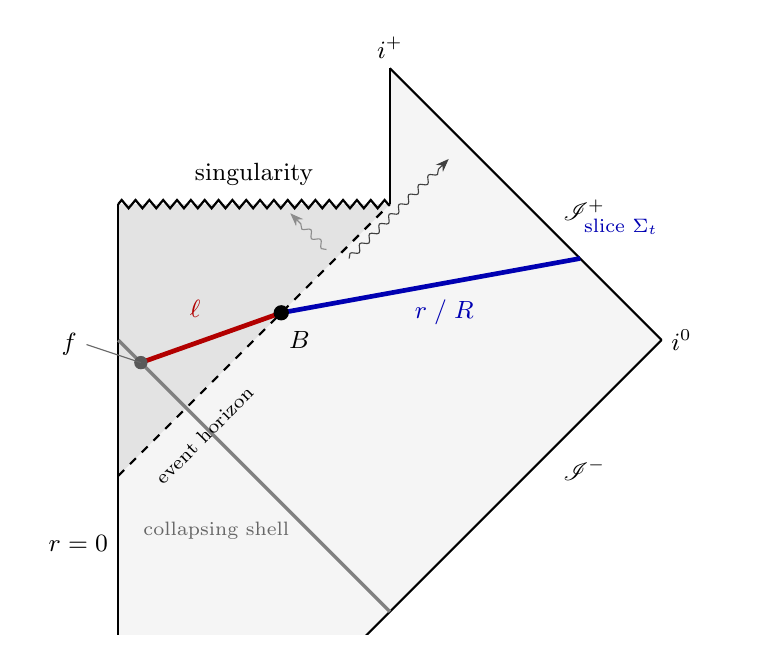
\begin{tikzpicture}[scale=1.15, >=Stealth, font=\small,
    quantum/.style={decorate, decoration={snake, amplitude=1.1pt, segment length=5pt, post length=3pt}, ->}]
  \clip (-1.0,2.75) rectangle (6.9,9.45);
  \coordinate (im) at (0,0);   \coordinate (iz) at (6,6);   \coordinate (ip) at (3,9);
  \coordinate (E) at (3,7.5);  \coordinate (S0) at (0,7.5);
  \fill[black!4] (im) -- (iz) -- (ip) -- (E) -- (S0) -- cycle;
  \fill[black!11] (0,4.5) -- (E) -- (S0) -- cycle;                       % black hole region
  \draw[thick] (im) -- (S0) node[pos=0.5, left] {$r=0$};
  \draw[thick] (E) -- (ip);
  \draw[thick] (im) -- (iz) node[pos=0.8, below right] {$\mathscr I^-$};
  \draw[thick] (iz) -- (ip) node[pos=0.4, above right] {$\mathscr I^+$};
  \draw[thick, decorate, decoration={zigzag, segment length=5pt, amplitude=1.5pt}] (S0) -- (E)
     node[midway, above=3pt] {singularity};
  \draw[very thick, black!50] (3,3) -- (0,6) node[pos=0.3, left=3pt, font=\scriptsize, black!60] {collapsing shell};
  \draw[thick, dashed] (0,4.5) -- (E);
  \node[font=\scriptsize, rotate=45] at (0.95,4.95) {event horizon};
  % one Hawking pair: outgoing quantum to I+, partner behind the horizon
  \draw[quantum, black!75] (2.55,6.9) -- (3.65,8.0);
  \draw[quantum, black!45] (2.3,7.0) -- (1.9,7.4);
  % Cauchy slice
  \coordinate (Ip) at (5.1,6.9); \coordinate (B) at (1.8,6.3); \coordinate (F) at (0.25,5.75);
  \draw[line width=1.7pt, blue!70!black] (Ip) -- (B);
  \draw[line width=1.7pt, red!70!black] (B) -- (F);
  \fill (B) circle (2.4pt); \fill[black!65] (F) circle (2.1pt);
  \node[blue!70!black, below] at (3.6,6.55) {$r\;/\;R$};
  \node[red!70!black] at (0.85,6.35) {$\ell$};
  \draw[black!60] (F) -- (-0.35,5.95) node[left, black] {$f$};
  \node at (2.0,6.0) {$B$};
  \node[blue!70!black, font=\scriptsize] at (5.55,7.25) {slice $\Sigma_t$};
  \node[right] at (iz) {$i^0$}; \node[above] at (ip) {$i^+$};
\end{tikzpicture}}

% ---------------------------------------------------------- two compressions
\newcommand{\CompressionPanel}[8]{% xshift, title, big, set, map, bigdim, small, smalldim
    \begin{scope}[xshift=#1 cm]
      \node[font=\small\bfseries] at (1.6,3.85) {#2};
      \draw[thick, fill=black!3] (1.6,1.75) ellipse (1.55 and 1.35);
      \node at (0.75,2.45) {$#3$};
      \node[font=\scriptsize, black!60] at (1.6,3.38) {$\dim=#6$};
      \fill[orange!35, draw=orange!70!black] plot[smooth cycle, tension=0.8]
        coordinates {(1.0,1.6) (1.5,2.15) (2.15,2.0) (2.3,1.45) (1.7,1.2)};
      \node at (1.65,1.65) {$#4$};
      \fill[pattern=north east lines, pattern color=black!35] (1.0,0.75) ellipse (0.55 and 0.25);
      \node[font=\scriptsize, black!60, anchor=west] at (1.6,0.55) {null states};
      \draw[thick, fill=black!3] (1.6,-1.25) ellipse (0.8 and 0.5);
      \node at (1.6,-1.25) {$#7$};
      \node[font=\scriptsize, black!60, anchor=west] at (2.45,-1.25) {$\dim=#8$};
      \draw[->, very thick] (1.6,0.35) -- node[right] {$#5$} (1.6,-0.7);
    \end{scope}}
\newcommand{\TwoCompressions}{%
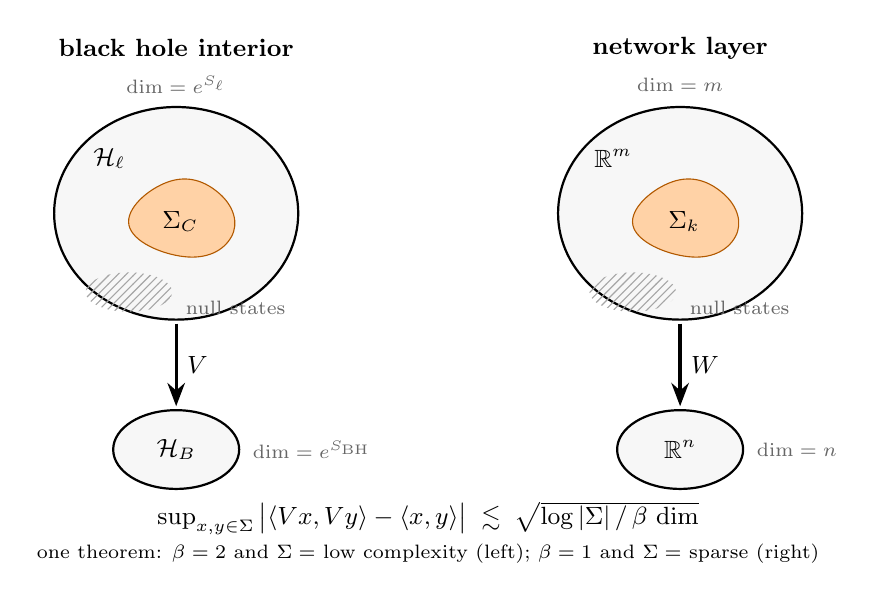
\begin{tikzpicture}[>=Stealth, font=\small]
  \CompressionPanel{0}{black hole interior}{\mathcal H_\ell}{\Sigma_C}{V}{e^{S_\ell}}{\mathcal H_B}{e^{S_{\rm BH}}}
  \CompressionPanel{6.4}{network layer}{\mathbb R^m}{\Sigma_k}{W}{m}{\mathbb R^n}{n}
  \node[align=center, font=\small] at (4.8,-2.3)
    {$\sup_{x,y\in\Sigma}\big|\langle Vx,Vy\rangle-\langle x,y\rangle\big| \;\lesssim\; \sqrt{\log|\Sigma|\,/\,\beta\,\dim}$\\[1pt]
     \scriptsize one theorem: $\beta=2$ and $\Sigma=$ low complexity (left); $\beta=1$ and $\Sigma=$ sparse (right)};
\end{tikzpicture}}

% ------------------------------------------------- toy model of superposition
\newcommand{\TMSPicture}{%
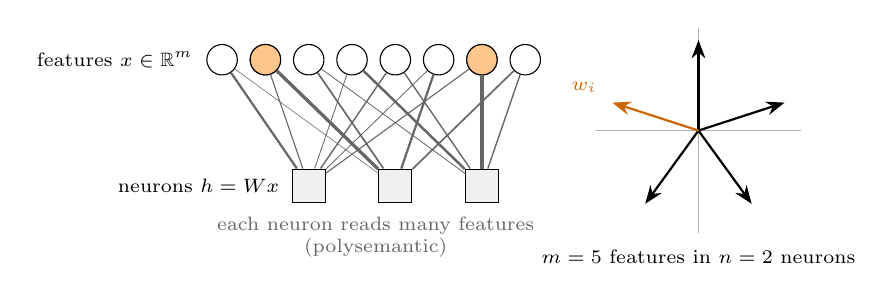
\begin{tikzpicture}[>=Stealth, font=\small, scale=1.0]
  % left: bipartite features -> neurons
  \foreach \i in {1,...,8} \node[circle, draw, minimum size=11pt, inner sep=0pt, fill=white] (f\i) at (0.55*\i,2.2) {};
  \foreach \i in {2,7} \node[circle, draw, minimum size=11pt, inner sep=0pt, fill=orange!45] at (f\i) {};
  \foreach \j in {1,2,3} \node[rectangle, draw, minimum size=12pt, inner sep=0pt, fill=black!6] (n\j) at (0.55+1.1*\j,0.6) {};
  \foreach \i/\j/\w in {1/1/0.8, 2/1/0.4, 2/2/1.2, 3/2/0.6, 4/3/0.9, 5/1/0.5, 5/3/0.5, 6/2/0.8, 7/3/1.2, 7/1/0.4, 8/2/0.6, 3/3/0.3, 6/1/0.3, 8/3/0.5, 1/2/0.2, 4/1/0.3}
     \draw[line width=\w pt, black!60] (f\i) -- (n\j);
  \node[anchor=east, font=\scriptsize] at (0.3,2.2) {features $x\in\mathbb R^m$};
  \node[anchor=east, font=\scriptsize] at (1.4,0.6) {neurons $h=Wx$};
  \node[font=\scriptsize, black!60, align=center] at (2.5,-0.05) {each neuron reads many features\\(polysemantic)};
  % right: pentagon of feature directions in R^2
  \begin{scope}[xshift=6.6cm, yshift=1.3cm]
    \draw[black!30] (-1.3,0) -- (1.3,0); \draw[black!30] (0,-1.3) -- (0,1.3);
    \foreach \k in {0,2,3,4} \draw[->, thick] (0,0) -- ({90+72*\k}:1.15);
    \draw[->, thick, orange!80!black] (0,0) -- (162:1.15);
    \node[font=\scriptsize] at (0,-1.6) {$m=5$ features in $n=2$ neurons};
    \node[font=\scriptsize, orange!80!black] at (-1.45,0.55) {$w_i$};
  \end{scope}
\end{tikzpicture}}

% ----------------------------------------------------- sender/receiver/monitor
\newcommand{\ChannelPicture}{%
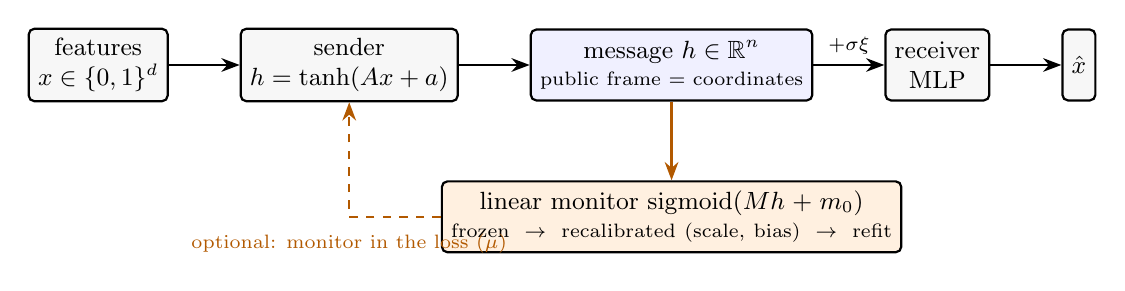
\begin{tikzpicture}[>=Stealth, font=\small, node distance=1.25cm,
    box/.style={draw, thick, rounded corners=2pt, minimum height=0.9cm, align=center, fill=black!3}]
  \node[box] (x) {features\\$x\in\{0,1\}^d$};
  \node[box, right=0.9cm of x] (s) {sender\\$h=\tanh(Ax+a)$};
  \node[box, right=0.9cm of s, fill=blue!6] (h) {message $h\in\mathbb R^n$\\[-1pt]\scriptsize public frame $=$ coordinates};
  \node[box, right=0.9cm of h] (r) {receiver\\MLP};
  \node[box, right=0.9cm of r] (xh) {$\hat x$};
  \draw[->, thick] (x) -- (s);
  \draw[->, thick] (s) -- (h);
  \draw[->, thick] (h) -- node[above, font=\scriptsize] {$+\sigma\xi$} (r);
  \draw[->, thick] (r) -- (xh);
  \node[box, below=1.0cm of h, fill=orange!12, text width=5.6cm] (m)
     {linear monitor $\mathrm{sigmoid}(Mh+m_0)$\\[-1pt]\scriptsize frozen $\;\to\;$ recalibrated (scale, bias) $\;\to\;$ refit};
  \draw[->, thick, orange!70!black] (h) -- (m);
  \draw[->, dashed, thick, orange!70!black] (m.west) -| (s.south);
  \node[font=\scriptsize, orange!70!black, anchor=north] at ($(s.south)+(0,-1.55)$) {optional: monitor in the loss ($\mu$)};
\end{tikzpicture}}

% ---------------------------------------------- legibility levels (ladder)
\newcommand{\MonitorLadder}{%
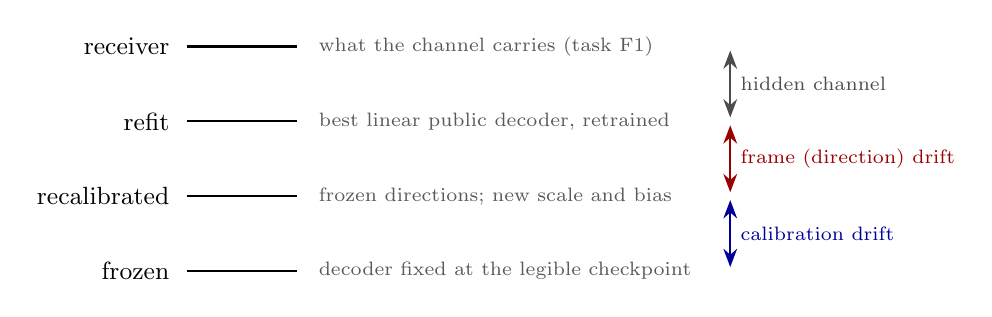
\begin{tikzpicture}[font=\small, >=Stealth]
  \foreach \y/\lab/\desc in {3/receiver/{what the channel carries (task F1)},
                             2/refit/{best linear public decoder, retrained},
                             1/recalibrated/{frozen directions; new scale and bias},
                             0/frozen/{decoder fixed at the legible checkpoint}} {
     \draw[thick] (0,0.95*\y) -- (1.4,0.95*\y);
     \node[anchor=east] at (-0.1,0.95*\y) {\lab};
     \node[anchor=west, font=\scriptsize, black!65] at (1.55,0.95*\y) {\desc};
  }
  \draw[<->, thick, blue!60!black] (6.9,0.05) -- node[right, font=\scriptsize, align=left] {calibration drift} (6.9,0.9);
  \draw[<->, thick, red!60!black] (6.9,1.0) -- node[right, font=\scriptsize, align=left] {frame (direction) drift} (6.9,1.85);
  \draw[<->, thick, black!70] (6.9,1.95) -- node[right, font=\scriptsize, align=left] {hidden channel} (6.9,2.8);
\end{tikzpicture}}


\title[Interpretability and the black hole interior]{Interpretability and the Black Hole Interior}
\author{David Wakeham and Claude}
\date{Version 0.1, November 2026. Written with Claude (Anthropic); see ``How these notes were made''.}

\begin{document}

\begin{abstract}
Neural networks simulate larger, interpretable networks using superposition. Black holes simulate the larger
Hilbert space of their interior using superposition. Part~I makes the resemblance precise: both are random
compressions that act as approximate isometries on ``thin'' sets of states (low complexity for the black hole,
sparsity for the network), and one theorem covers both. From it we build a dictionary between the physics of the
interior (null states, state-dependent reconstruction, the Page transition, the Python's lunch) and feature
recovery as compressed sensing, with an explicit list of where the dictionary is exact and where it is only
analogy. We then test the randomness assumption on trained models: toy models of superposition, RoBERTa token
embeddings and GloVe. Trained codes agree with Haar-random codes at second order---but a frame identity forces
this for any tight frame---and differ in informative ways at fourth order, in anisotropy and in their tails, while
still recovering sparse combinations at the Donoho--Tanner threshold. Part~II asks what training does to the
\emph{orientation} of a code relative to a public frame, the property that monitoring depends on. In a toy
sender--receiver model, a code that is legible in the public frame is a critical point of the training loss when its
coordinates are unshared. Theory makes it a saddle whose curvature is proportional to the receiver's residual error;
at our operating point that curvature is below $10^{-9}$, and what moves the code is that adaptive optimizers turn
vanishing gradients into finite steps. Accordingly, plain SGD on the sender alone preserves legibility at no cost to
the task, while Adam spreads the code to no benefit. In superposition the legible code is not a critical point,
drift follows the receiver, and the optimizer prescription fails. A quantitative test of the curvature theory was
confounded by the receiver memorizing its training noise. Several claims from earlier drafts did not survive the experiments; the corrections are listed.
\end{abstract}

\maketitle

\begin{tcolorbox}[colback=black!3, colframe=black!40, title=How these notes were made, fonttitle=\bfseries\small, fontupper=\small]
The idea of comparing the non-isometric code of Akers, Engelhardt, Harlow, Penington and Vardhan~\cite{AEHPV}
with superposition in neural networks, the decision to pursue its consequences for monitoring agents that
communicate in activations, and the editorial direction of these notes are David Wakeham's. The derivations,
code, experiments and most of the prose were produced by Claude (Anthropic; Claude Opus models) in conversation
with D.W.\ between September and November 2026, with D.W.\ choosing directions, asking for checks, and editing.
Every number in these notes is produced by a script in the accompanying repository (\repo; see
\cref{app:repro}). Claims carry a status tag: \proved\ (proof given here), \cited\ (standard result, reference
given), \numchk\ (verified by the code but not proved), \heur\ (derivation with uncontrolled steps), or
\analogy. Earlier versions of several Part~II claims were wrong; \cref{app:corrections} lists what changed and
which experiment changed it. \emph{Author's verification status:} at the time of writing D.W.\ has not yet
independently checked every derivation; this sentence will be updated as he does.
\end{tcolorbox}
\newpage
\tableofcontents
\newpage
\section{Introduction}\label{sec:intro}

Black holes, like neural networks, are hard to look inside: a black hole has a horizon; a neural network is
polysemantic. We show this is more than a simile. In both cases, a large ``effective'' space (the black hole
interior; feature space) is compressed by a linear map into a smaller ``fundamental'' space (microscopic degrees
of freedom; physical neurons). This forces initially orthogonal directions to overlap, leading to null states and
state-dependent operators in the black hole setting, and interference and polysemanticity in networks. We isolate a
single condition for the validity of both effective descriptions: states or features form an appropriately
``thin'' set for which random linear compressions preserve inner products. We use this to build a correspondence
between black holes and neural networks, make quantitative predictions about feature recovery, and test them in
toy models of superposition and in the embeddings of trained language models. A collapsed star is a surprisingly
rich guide to the inside of a neural network.

\begin{figure}[t]
\centering\TwoCompressions
\caption{The two compressions. A large effective space is mapped by a linear code into a much smaller
fundamental space. Most of the large space is annihilated (null states), yet on a thin set $\Sigma$---low
complexity on the left, sparsity on the right---inner products survive. \Cref{thm:main} is the statement that
these are one phenomenon.}
\label{fig:two}
\end{figure}

Of the parallels, the Python's lunch~\cite{Lunch} deserves mention, because it concerns an
\emph{observer} rather than the code. A lunch is a region whose information is present in the fundamental
description but whose reconstruction is exponentially complex. Its classical counterpart is the gap between
statistical and computational recovery in sparse decoding. A monitor is also an observer---a decoder with a fixed
frame and a bounded budget---and this is where Part~II begins. For a black hole the code is a fixed fact about a
state. For a network it is trained, so the question becomes dynamical: does optimization keep representations
legible to a monitor, or move them away? Part~II studies this in the smallest model where the question makes
sense.

\subsection*{Summary of findings}
\begin{enumerate}[leftmargin=*, itemsep=2pt]
\item \textbf{One theorem} \proved. A Haar-random code over $\F\in\{\R,\C\}$ from dimension $M$ to $N$ preserves
all inner products on a set $\Sigma$ to accuracy $\delta$ once $\log\abs{\Sigma}\ll\beta N\delta^2$
(\cref{thm:main}). Low circuit complexity (AEHPV) and sparsity (the
restricted isometry property from compressed sensing) are two special cases.
\item \textbf{Exact moments} \proved\ \numchk. Overlap variances are $\frac{(M-N)(M-\abs{c}^2)}{N(M^2-1)}$ over
$\C$ and $\frac{(m-n)(m+(m-2)c^2)}{n(m-1)(m+2)}$ over $\R$; the real/complex difference is exactly the third
Brauer invariant (\cref{lem:projectors}).
\item \textbf{Trained codes are not Haar, but are ``Haar-good''} \numchk. Second moments agree for a reason
unrelated to randomness (\cref{prop:frame-identity}). Toy-model codes are \emph{better} than Haar at the extremes
when features are plentiful, and maximally non-Haar (antipodal) when they are not. Real embeddings are
anisotropic with heavy-tailed overlaps. Yet $\ell_1$ recovery of random sparse combinations sits at the Haar threshold, as the known universality of the
Donoho--Tanner transition~\cite{Monajemi} would lead one to expect (\cref{sec:part1-exp}).
\item \textbf{Legibility is a critical point, where there is room} \heur\ \numchk. In a sender--receiver toy, a
code that is sparse in the public frame is a critical point in ``leak'' directions toward empty coordinates. Theory
makes it a saddle with curvature proportional to the receiver's residual error (\cref{sec:saddle}); at our operating
point that curvature is below $10^{-9}$, so the point is a plateau, and what matters is that Adam turns vanishing
gradients into finite steps while gradient descent does not move. Accordingly, plain SGD on the sender alone keeps
features on their coordinates at no cost to the task, even with Adam elsewhere---but only when coordinates are
unshared. In superposition the legible code is not a critical point, drift follows the receiver, and the prescription
fails. The quantitative curvature theory is untested in the full model (\cref{sec:part2-exp}).
\item \textbf{Corrections} \numchk. Most of the frozen-monitor degradation reported in earlier drafts is
\emph{calibration} drift, repairable by refitting a scale and bias per feature. The residual directional drift is
real but smaller. Raising task pressure did not spread the code, and putting the monitor in the loss did not open a
hidden channel at this scale (\cref{sec:part2-exp}, \cref{app:corrections}).
\end{enumerate}

\part*{Part I.\quad The correspondence}
% ============================================================== PART I
\section{Two compressions}\label{sec:two}

\subsection{The black hole interior}\label{sec:bh}
The literature on the quantum mechanics of black holes is enormous; the part we need concerns Hawking's information
paradox and its recent resolution through holography~\cite{Penington,AEMM,AEHPV}. In particular, we exploit the
insight of Akers, Engelhardt, Harlow, Penington and Vardhan~\cite{AEHPV} that the effective description of the
black hole interior---the ``bulk'' local physics, such as the creation and annihilation operators of quantum fields
inside the horizon---is related to the fundamental description by a random linear compression. The fundamental
description consists of the black hole's own remaining degrees of freedom, counted by its entropy, together with the
radiation it has emitted; the compression acts on the interior modes alone and carries the radiation across
untouched (\cref{fig:penrose}). This single picture accounts for several pieces of black hole folklore: the Page
curve of the radiation entropy, the state-dependence of interior operators, the absence of low-complexity null
states, and the exponential cost of decoding the radiation.

\begin{figure}[t]
\centering\PenroseSlice
\caption{Late-time Cauchy slice $\Sigma_t$ of an evaporating black hole formed by a collapsing shell (zoomed on the
relevant region; null lines at $45^\circ$). Outside the horizon the slice carries the outgoing Hawking modes $r$,
which are the same system $R$ in both descriptions. Inside, it carries the infalling partner modes $\ell$ near the
horizon and, at its inner end, the collapsed matter $f$, frozen in the state it fell in with. In the fundamental
description the whole interior segment is encoded in the black hole's microstates $B$ at the horizon crossing, with
$\dim\Hil_B=e^{A/4G}$: the map $V$ squeezes a segment onto a point whose size is its area. Lower-case labels are
what a semiclassical observer assigns to a region; upper-case labels are the fundamental Hilbert spaces. They differ
only at the horizon, and the difference is $V$.}
\label{fig:penrose}
\end{figure}

Formally, we can forget about gravity and time evolution and focus on the linear algebra of inner-product spaces.
The effective description of the interior is a Hilbert space $\Hil_\ell$ of dimension $\abs{\ell}=e^{S_\ell}$; at
late times $S_\ell$ exceeds the black hole's Bekenstein--Hawking entropy $S_{\rm BH}$, because the interior keeps
growing while the black hole shrinks. The fundamental description of the black hole is $\Hil_B$ with
$\abs{B}=e^{S_{\rm BH}}$. The two are related by
\begin{equation}\label{eq:V}
V\colon\Hil_\ell\to\Hil_B,\qquad V=\sqrt{\abs{P}}\;\bra{0}_P\,U\,\ket{\psi_0}_f ,\qquad \abs{\ell}\abs{f}=\abs{B}\abs{P},
\end{equation}
extended by the identity on the radiation. Here $U$ is a Haar-random unitary on $\Hil_\ell\otimes\Hil_f$ standing
in for the unknown, scrambling dynamics; $f$ is the collapsed matter, prepared in a fixed state $\ket{\psi_0}$ by the
history of the collapse; and $P$ is a bookkeeping remainder. The interior $\ell\otimes f$ has more states than the
black hole $B$ can hold, so the unitary must output them somewhere: $P$ is that somewhere, discarded by projection
onto $\ket 0_P$---the states the black hole would have needed had it not shrunk.

The factor $\sqrt{\abs P}$ makes typical states come out with unit norm. Indeed
$\bra0_PU\ket{\psi_0}_f$ is a block of $U$, and $U^\dagger(I_B\otimes\ket0\bra0_P)U$ is a Haar-random projector of
rank $\abs B$ on a space of dimension $\abs\ell\abs f=\abs B\abs P$, so by \cref{lem:projectors},
$\E\,V^\dagger V=\abs P\cdot\frac{\abs B}{\abs\ell\abs f}\,I_\ell=I_\ell$.

For the linear algebra the ancillae are inessential and we use the \emph{reduced model} $\abs f=1$:
\begin{equation}\label{eq:reduced}
V=\sqrt{M/N}\;P_NU,\qquad M=\abs\ell,\ N=\abs B,
\end{equation}
$\sqrt{M/N}$ times $N$ rows of a Haar unitary. Then $V^\dagger V=\frac MN Q$ with $Q$ a Haar-random rank-$N$
projector. Since $M>N$, $\dim\ker V\ge M-N$: almost all of the effective space consists of \emph{null states}
that the fundamental description cannot distinguish from zero. The content of~\cite{AEHPV} is that $V$ is
nonetheless an isometry to any observer of bounded complexity; \cref{sec:theorem} proves the version we need.

\subsection{Superposition}\label{sec:superposition}
The working hypothesis of mechanistic interpretability is that a trained network computes with \emph{features}:
directions in activation space that correspond to human-legible properties of the input. The obstacle is that
features are not neurons. A neuron typically responds to several unrelated features and a feature is spread across
many neurons---\emph{polysemanticity}. Elhage et al.~\cite{TMS} showed that polysemanticity is what compression
looks like from the inside. A network that must represent $m$ features in $n<m$ neurons can, if the features are
sparse, assign each a direction in $\R^n$ and accept that the directions overlap, because overlaps only matter
when overlapping features are simultaneously active. This is \emph{superposition}: the network simulates a larger,
monosemantic network (\cref{fig:tms}).

\begin{figure}[t]
\centering\TMSPicture
\caption{Superposition. Left: $m$ features feed $n<m$ neurons; a sparse input (shaded) activates few features but
every neuron reads several. Right: the classic toy-model solution with $m=5$ features in $n=2$ dimensions, a
regular pentagon~\cite{TMS}.}
\label{fig:tms}
\end{figure}

The effective description is feature space $\R^m$; a feature activation $x$ is nonzero on few coordinates, and we
write $\Sigma_k$ for the unit vectors with at most $k$ nonzero entries. The fundamental description is the
activation space $\R^n$. The two are related by $W\colon\R^m\to\R^n$, $h=Wx$, whose columns $w_1,\dots,w_m$ are the
feature directions. In the toy models of~\cite{TMS} the readout is $\hat x=\ReLU(W^\top h+b)$. The transpose alone
cannot undo superposition (any linear map $\R^n\to\R^m$ has rank $\le n$); $W^\top Wx=x+e$ is correct on the active
coordinates up to the \emph{interference} $e_i=\sum_{j\ne i}\ip{w_i}{w_j}x_j$, and the ReLU with negative bias
projects back onto the sparse set by thresholding the interference away (\cref{prop:onestep}). Since $m>n$, $W$
cannot be an isometry; its kernel contains the dense activation patterns that a sparse network never produces.

\subsection{The static dictionary}
\Cref{tab:static} lines up the two settings. The quantitative content of ``preserves inner products on a
distinguished set'' is the subject of \cref{sec:theorem}. The one structural asymmetry is that $V$ is assembled
from a unitary with ancillae, because in gravity the scrambling is unitary and the compression has to be
manufactured from it, whereas $W$ is trained directly; nothing in the dictionary depends on the ancillae.

\begin{table}[h]
\centering\small
\begin{tabular}{@{}lll@{}}
\toprule
 & black hole (AEHPV) & network (superposition) \\
\midrule
effective space & interior $\Hil_\ell$, $\dim=e^{S_\ell}$ & features $\R^m$ \\
fundamental space & microstates $\Hil_B$, $\dim=e^{S_{\rm BH}}$ & neurons $\R^n$ \\
code & $V$, from a Haar unitary & $W$, trained (Haar as baseline) \\
null space & $\dim\ge M-N$, all high complexity & $\ker W$, no $k$-sparse vectors \\
distinguished set & complexity $\le C$ & $k$-sparse \\
its size & $\log\abs{\Sigma_C}\lesssim C\log S_\ell$ & $\log\binom mk\le k\log(em/k)$ \\
overlap fluctuations & $\approx e^{-S_{\rm BH}/2}$ & $\approx n^{-1/2}$ \\
field & $\C$ ($\beta=2$) & $\R$ ($\beta=1$) \\
\bottomrule
\end{tabular}
\caption{The static dictionary. The exponential in the left column becomes polynomial on the right:
$e^{S_{\rm BH}}\leftrightarrow n$, hence $S_{\rm BH}\leftrightarrow\log n$.}
\label{tab:static}
\end{table}

% --------------------------------------------------------------------------
\section{The unifying theorem}\label{sec:theorem}

Throughout, a code maps an $M$-dimensional effective space to an $N$-dimensional fundamental space over
$\F\in\{\R,\C\}$; write $\beta=\dim_\R\F$. The \emph{Haar code} is $V=\sqrt{M/N}\,P_NU$ with $U$ Haar on $U(M)$
(complex) or $O(M)$ (real); in the real case we write $W$, $m$, $n$. For a set $\Sigma$ of unit vectors the
distortion is $\epsilon_\Sigma(V)=\sup_{x,y\in\Sigma}\abs{\ip{Vx}{Vy}-\ip xy}$.

\subsection{Second moments}
\begin{lemma}[Projector moments]\label{lem:projectors}\proved
Let $Q$ be a Haar-random rank-$N$ orthogonal projector on $\F^M$. Then $\E Q=\frac NM I$, and
\begin{align*}
\F=\C:&\quad \E[Q\otimes Q]=aI+bF, & a&=\tfrac{N(NM-1)}{M(M^2-1)},\ \ b=\tfrac{N(M-N)}{M(M^2-1)};\\
\F=\R:&\quad \E[Q\otimes Q]=\alpha I+\gamma(F+\Omega), & \gamma&=\tfrac{N(M-N)}{M(M-1)(M+2)},\ \ \alpha=\tfrac NM-\gamma(M+1),
\end{align*}
where $F$ is the swap and $\Omega=\ket\omega\bra\omega$ with $\ket\omega=\sum_ie_i\otimes e_i$.
\end{lemma}
\begin{proof}
$\E Q$ commutes with every unitary (orthogonal) $g$, since $g^\dagger Qg$ has the same law as $Q$; so $\E Q=cI$ and
$\tr$ gives $c=N/M$. Likewise $\E[Q\otimes Q]$ commutes with all $g\otimes g$. Over $\C$ the commutant of
$\{g\otimes g\}$ is spanned by $I,F$ (Schur--Weyl); over $\R$ by $I,F,\Omega$ (Brauer). Fix the coefficients by
traces. Over $\C$: $\tr\E[Q\otimes Q]=(\tr Q)^2=N^2=aM^2+bM$ and $\tr(F\,\E[Q\otimes Q])=\tr Q^2=N=aM+bM^2$, which
solve to the stated $a,b$. Over $\R$ there is a third equation, $\tr(\Omega\,\E[Q\otimes Q])=\tr(QQ^\top)=N$; using
$\tr F=\tr\Omega=M$, $\tr(F\Omega)=M$, $\tr F^2=\tr\Omega^2=M^2$, the second and third equations are symmetric in the
coefficients of $F$ and $\Omega$, so these are equal ($=\gamma$), and $N^2=\alpha M^2+2\gamma M$,
$N=\alpha M+\gamma(M^2+M)$ give $\gamma M(M-1)(M+2)=N(M-N)$.
\end{proof}

\begin{proposition}[Exact overlap variances]\label{prop:variances}\proved\ \numchk
For fixed unit vectors with overlap $c$, $\E\ip{Vx}{Vy}=c$ and
\[
\Var_{\C}=\frac{(M-N)(M-\abs c^2)}{N(M^2-1)},\qquad
\Var_{\R}=\frac{(m-n)\,\big(m+(m-2)c^2\big)}{n\,(m-1)(m+2)},\qquad
\Var_{\rm Gauss}=\frac{1+c^2}{n},
\]
the last for i.i.d.\ $\mathcal N(0,1/n)$ entries. For $N\ll M$ the complex variance is $\approx1/N$ independently of
$c$; the real one is $\approx(1+c^2)/n$, and the extra $c^2$ is exactly the $\Omega$ term of \cref{lem:projectors},
the Brauer invariant that is present for $O(n)$ and absent for $U(n)$. Haar frames beat Gaussian ones by a factor
$\approx(1-n/m)$.
\end{proposition}
\begin{proof}
$\E\abs{\bra x Q\ket y}^2=(\bra x\otimes\bra y)\E[Q\otimes Q](\ket y\otimes\ket x)=a\abs c^2+b$ over $\C$; over $\R$,
$\E(x^\top Qy)^2=(\alpha+\gamma)c^2+\gamma$. Multiply by $(M/N)^2$, subtract $\abs c^2$, simplify. For Gaussian
entries apply Isserlis to the $n$ independent terms $\ip{g_i}x\ip{g_i}y$.
\end{proof}

\begin{proposition}[Frame identity]\label{prop:frame-identity}\proved
Let $w_1,\dots,w_m$ be unit vectors in $\R^n$ forming a tight frame ($WW^\top=\frac mn I$). Then
\[
\frac{1}{m(m-1)}\sum_{i\ne j}\ip{w_i}{w_j}^2=\frac{m-n}{n(m-1)} .
\]
Hence \emph{every} unit-norm tight frame agrees with the Haar prediction $\frac{m(m-n)}{n(m-1)(m+2)}$ for the
mean-square interference, up to a factor $m/(m+2)$.
\end{proposition}
\begin{proof}
$\sum_{i,j}\ip{w_i}{w_j}^2=\norm{W^\top W}_F^2=\norm{WW^\top}_F^2=(m/n)^2n$; subtract the $m$ diagonal terms.
\end{proof}
This matters for experiments: agreement with Haar at second order is evidence of tightness, not of randomness.

\subsection{Concentration and the theorem}
\begin{lemma}[Law of a compressed norm]\label{lem:beta}\proved
For fixed unit $z$, $\norm{Vz}^2\overset{d}{=}\frac MN\cdot\frac{A}{A+B}$ with $A\sim\chi^2_{\beta N}$,
$B\sim\chi^2_{\beta(M-N)}$ independent.
\end{lemma}
\begin{proof}
$\norm{Vz}^2=\frac MN\norm{P_NUz}^2$ and $Uz$ is uniform on the unit sphere of $\F^M\cong\R^{\beta M}$, i.e.\ $g/\norm
g$ with $g$ standard Gaussian. $\norm{P_Ng}^2\sim\chi^2_{\beta N}$ and $\norm{(1-P_N)g}^2\sim\chi^2_{\beta(M-N)}$
independently.
\end{proof}

\begin{lemma}[$\chi^2$ concentration]\label{lem:chisq}\proved
For $Z\sim\chi^2_k/k$ and $0<s\le1$: $\Pr[\abs{Z-1}\ge s]\le2e^{-ks^2/12}$.
\end{lemma}
\begin{proof}
Chernoff with $\E e^{\lambda\xi^2}=(1-2\lambda)^{-1/2}$. Upper tail: $\lambda=\frac{s}{2(1+s)}$ gives exponent
$-\frac k2[s-\log(1+s)]\le-\frac{k}{2}(\frac{s^2}{2}-\frac{s^3}{3})\le-\frac{ks^2}{12}$. Lower tail:
$\lambda=\frac{s}{2(1-s)}$ for the variable $-\xi^2$ gives exponent $-\frac k2[-s-\log(1-s)]\le-\frac{ks^2}{4}$.
\end{proof}

\begin{theorem}[Random codes are isometries on thin sets]\label{thm:main}\proved
Let $V$ be the Haar code over $\F$ and $T$ a finite set of unit vectors. For $0<\delta\le1$,
\[
\Pr\Big[\sup_{z\in T}\big|\norm{Vz}^2-1\big|>\delta\Big]\le4\abs T\,e^{-\beta N\delta^2/108}.
\]
Consequently, for any finite set $\Sigma$ of unit vectors, $\epsilon_\Sigma(V)\le2\delta$ with probability at least
$1-16\abs\Sigma^2e^{-\beta N\delta^2/108}$; that is, the code is an approximate isometry on $\Sigma$ as soon as
\begin{equation}\label{eq:condition}
\boxed{\;\log\abs\Sigma\;\ll\;\beta\,N\,\delta^2\;}
\end{equation}
\end{theorem}
\begin{proof}
By \cref{lem:beta}, $\norm{Vz}^2=\frac{A/\beta N}{(A+B)/\beta M}$. If numerator and denominator are both within
$1\pm\delta/3$ the ratio is within $1\pm\delta$ (since $\frac{1+t}{1-t}\le1+3t$ for $t\le\frac13$), and by
\cref{lem:chisq} each fails with probability at most $2e^{-\beta N\delta^2/108}$. Union-bound over $T$. For the
second statement apply this to $T=\{(x+\omega y)/\norm{x+\omega y}\}$ with $\omega\in\{\pm1\}$ (real) or
$\{\pm1,\pm i\}$ (complex), $\abs T\le4\abs\Sigma^2$, and use polarization:
$\abs{\ip{Vx}{Vy}-\ip xy}\le\frac14\sum_\omega\delta\norm{x+\omega y}^2\le2\delta$.
\end{proof}

The theorem never asks which field or which set it is given; it sees only $\beta$ and $\log\abs\Sigma$. Its two
specializations are the two halves of the correspondence.

\begin{corollary}[AEHPV: low complexity]\label{cor:aehpv}\proved
Over $\C$ with $N=e^{S_{\rm BH}}$, let $\Sigma_C$ be the states preparable from a fixed reference state by circuits of
at most $C$ gates from a finite gate set $G$ acting on the $S_\ell$ interior qubits. Then
$\abs{\Sigma_C}\le(\abs G S_\ell^2)^C$, and with high probability
\[
\sup_{\psi,\phi\in\Sigma_C}\big|\bra\psi V^\dagger V\ket\phi-\braket\psi\phi\big|\lesssim\sqrt{C\log S_\ell}\;e^{-S_{\rm BH}/2},
\]
negligible for all $C$ sub-exponential in $S_{\rm BH}$. In particular no state of sub-exponential complexity is null.
\end{corollary}

\begin{corollary}[Restricted isometry]\label{cor:rip}\proved
Over $\R$, $W$ satisfies $(1-\delta)\le\norm{Wx}^2\le(1+\delta)$ for all $k$-sparse unit $x$ with high probability
once $n\gtrsim\delta^{-2}k\log(em/k)$.
\end{corollary}
\begin{proof}
For each support $S$ take an $\eta$-net of the unit sphere of $\R^S$ with at most $(3/\eta)^k$ points; the union
over $\binom mk$ supports has $\log\abs T\le k\log(em/k)+k\log(3/\eta)$. Apply \cref{thm:main} to the net, then
extend from the net to the sphere: if $1-\delta'\le\norm{Wz}\le1+\delta'$ on the net and $A=\sup\norm{Wz}$, then
$A\le1+\delta'+\eta A$, so $A\le(1+\delta')/(1-\eta)$, and similarly from below; take $\eta=\delta'/4$.
\end{proof}

\begin{remark}[No simple null vectors]
If $\delta_{2k}<1$ then no nonzero $2k$-sparse vector is in $\ker W$, so $\spark(W)>2k$ and each $k$-sparse vector
is determined by its image. The dictionary entry is: $\spark(W)$ is the complexity of the cheapest null state.
\end{remark}

\begin{remark}[Gaussian width]\label{rem:width}\cited
The finite-set condition $\log\abs\Sigma\ll\beta N\delta^2$ is the special case of Gordon's
theorem~\cite{Gordon,Vershynin}: a Gaussian $n\times m$ map is an approximate isometry on any $T\subset S^{m-1}$
with distortion $\lesssim w(T)/\sqrt n$, where $w(T)=\E\sup_{z\in T}\ip gz$. For finite sets $w(T)\le\sqrt{2\log\abs
T}$ (Jensen on $\E\max e^{\lambda\ip gz}$), and for the $k$-sparse sphere
$w(\Sigma_k)\le\sqrt k+\sqrt{2\log\binom mk}$ (the same argument applied to the 1-subgaussian variables
$\norm{g_S}-\E\norm{g_S}$, with $\E\norm{g_S}\le\sqrt k$). Width is the right size for $\Sigma$; low complexity and
sparsity are two ways of having small width. We do not need the complex version of Gordon's theorem, because both
corollaries above go through the finite-set form.
\end{remark}

\begin{remark}[Where the exponential goes]
Gravity compares $\mathrm{poly}(C)$ with $e^{S_{\rm BH}}$; a network compares $k\log(m/k)$ with $n$. The dictionary
is $e^{S_{\rm BH}}\leftrightarrow n$, so corrections that are $e^{-S/2}$ in gravity are $n^{-1/2}$ in a network,
and an effective description that is quasi-exact for a black hole is merely approximate for a transformer. This is
the largest quantitative deflation in passing from one column of \cref{tab:static} to the other.
\end{remark}

% --------------------------------------------------------------------------
\section{The reconstruction dictionary}\label{sec:dictionary}

\subsection{Decoders}
On both sides the naive decoder is the adjoint of the encoder: the Petz (transpose) map~\cite{Petz} in gravity,
$W^\top$ followed by a nonlinearity in a network.
\begin{lemma}\proved
If $\epsilon_\Sigma(V)\le\epsilon$ then $\abs{\ip y{V^\dagger Vx}-\ip yx}\le\epsilon$ for all $x,y\in\Sigma$.
\end{lemma}
That is all one can say: $V^\dagger Vx$ agrees with $x$ against every test vector in $\Sigma$ and may be badly wrong
elsewhere. In a network this ``elsewhere'' is the interference, and the nonlinearity's job is to project back to
$\Sigma$.
\begin{proposition}[One-step thresholding]\label{prop:onestep}\proved
If the columns of $W$ are unit vectors with coherence $\mu=\max_{i\ne j}\abs{\ip{w_i}{w_j}}$ and $x\in\{0,1\}^m$ has
at most $k$ ones, then $\abs{(W^\top Wx)_i-x_i}\le\mu k$; so $\ReLU(W^\top Wx-\frac12)$ followed by rounding
recovers $x$ when $\mu k<\frac12$.
\end{proposition}
For random unit columns $\mu\approx\sqrt{2\log m/n}$, so one step tolerates $k\lesssim\sqrt{n/\log m}$, whereas the
isometry holds up to $k\sim n/\log(m/k)$; iterative and convex decoders close the gap (\cref{sec:page}).

\subsection{State dependence}\label{sec:state-dependence}
\begin{proposition}[Why reconstruction must be state-dependent]\label{prop:statedep}\proved
In the reduced model, for any operator $A$ on the effective space,
\[
\E\big[V^\dagger V\,A\,V^\dagger V\big]=\frac{M(NM-1)}{N(M^2-1)}\,A+\frac{M(M-N)}{N(M^2-1)}\,\tr(A)\,I\;\approx\;A+\frac{\tr A}{N}\,I .
\]
So the state-independent reconstruction $VAV^\dagger$ has, in every state $V\ket\phi$, an expectation biased by
$\approx e^{-S_{\rm BH}}\tr A$. For $A=I$ the reconstruction $VV^\dagger$ has expectation exactly
$\frac MN\bra\phi V^\dagger V\ket\phi\approx e^{S_\ell-S_{\rm BH}}$: the fundamental description of the identity is
not even approximately the identity. A state-dependent reconstruction $A_\phi$ defined by $A_\phi V\ket\phi=VA\ket\phi$
inherits the accuracy of \cref{cor:aehpv} whenever $\ket\phi$, $A\ket\phi$ and $B\ket\phi$ are low-complexity.
\end{proposition}
\begin{proof}
Index computation with \cref{lem:projectors}: $\E[QAQ]_{ij}=\sum_{kl}\E[Q_{ik}Q_{lj}]A_{kl}=aA_{ij}+b\,\delta_{ij}\tr A$;
multiply by $(M/N)^2$. For $A=I$ use $(V^\dagger V)^2=\frac MNV^\dagger V$. The last statement is
$\bra\phi V^\dagger B_\phi^\dagger A_\phi V\ket\phi=\ip{VB\phi}{VA\phi}$ and \cref{cor:aehpv}.
\end{proof}
The mechanism is instructive. $\Delta=V^\dagger V-I$ has small matrix elements between low-complexity states, but
$\norm{\Delta\phi}^2\approx M/N-1$ is huge: the error vector points entirely in high-complexity directions, which no
low-complexity test vector sees. $VAV^\dagger$ sandwiches $A$ between two such vectors. The network analogue is a
decoder fitted on one distribution over $\Sigma$, which fails silently on another.

\subsection{The Page transition and the Donoho--Tanner transition}\label{sec:page}
\begin{proposition}[Lubkin; R\'enyi-2 Page curve]\proved\ \numchk
For a Haar-random pure state on $\C^{d_A}\otimes\C^{d_B}$, $\E\tr\rho_A^2=\frac{d_A+d_B}{d_Ad_B+1}$.
\end{proposition}
\begin{proof}
$\ket\Psi\bra\Psi$ is a Haar rank-one projector, so $\E\ket\Psi\bra\Psi^{\otimes2}=\frac{I+F}{M(M+1)}$ by
\cref{lem:projectors}; $\tr\rho_A^2=\tr[(F_A\otimes I)\ket\Psi\bra\Psi^{\otimes2}]$ and the two traces give
$d_Ad_B^2+d_A^2d_B$.
\end{proof}
Subsystem $A$ is maximally mixed until it is more than half the system: the transition sits at $\log d_A=\log d_B$,
an equality of two entropies, which in the gravitational description is the crossover of two quantum extremal
surfaces~\cite{Penington,AEMM}.

On the classical side, basis pursuit $\hat x=\arg\min\{\norm z_1:Wz=Wx\}$ returns $x$ if and only if
$\ker W\cap D(\norm\cdot_1,x)=\{0\}$, where $D$ is the descent cone \proved. A random kernel misses a fixed cone with
overwhelming probability when $n>\sdim(D)$ and hits it when $n<\sdim(D)$, with a window of width
$O(\sqrt m)$~\cite{ALMT} \cited. The statistical dimension is computable:
\begin{proposition}[Location of the transition]\label{prop:sdim}\proved\ \numchk
For $x$ with $k=\rho m$ nonzero entries,
$\sdim(D)/m\le\psi(\rho)=\inf_{\tau\ge0}\{\rho(1+\tau^2)+(1-\rho)\,2[(1+\tau^2)\Phi(-\tau)-\tau\varphi(\tau)]\}$,
tight up to $O(1/\sqrt m)$. For nonnegative $x$ recovered by $\min\{\sum z: Wz=Wx,\ z\ge0\}$ the factor $2$ is
absent (only the upper tail of the off-support coordinates contributes), giving $\psi_+(\rho)$.
\end{proposition}
\begin{proof}
$D^\circ=\cone(\partial f(x))$, so $\sdim(D)=\E\,\mathrm{dist}(g,\cone\,\partial f)^2\le\inf_\tau\E\,\mathrm{dist}(g,\tau\partial f)^2$.
For $\norm\cdot_1$ the distance splits coordinatewise into $(g_i-\tau\,\mathrm{sign}\,x_i)^2$ on the support and
$(\abs{g_i}-\tau)_+^2$ off it; $\E(g-\tau)_+^2=(1+\tau^2)\Phi(-\tau)-\tau\varphi(\tau)$. For the nonnegative problem the
subdifferential off the support is $\{u\le1\}$, so only $(g_i-\tau)_+^2$ appears.
\end{proof}
Solving $m\psi(k/m)=n$ gives the Donoho--Tanner curve~\cite{DT}. In our code, $n=40$, $m=120$ gives $k^*=12.2$
(signed) and $17.2$ (nonnegative); simulated 50\% crossings are at $k\approx12.5$ and $18$.

\begin{entry}[Page $\leftrightarrow$ Donoho--Tanner; QES crossover $\leftrightarrow$ ALMT edge]\analogy\ (structural)
Both are typicality statements about a Haar or Gaussian object, both are sharp in large dimension, and both are
located by an equality between two dimension-like functionals---one measuring what is available, one measuring what
must be resolved. What the parallel is \emph{not}: there is no extremization principle on the classical side.
The QES prescription minimizes over candidate surfaces; $\sdim(D)$ is a single number attached to a cone.
\end{entry}

\subsection{The Python's lunch and the computational--statistical gap}
Every $k$-sparse $x$ is determined by $Wx$ iff $\spark(W)>2k$, and a Gaussian $W$ has $\spark=n+1$ almost surely,
so $n\ge2k$ suffices \proved. The decoder this implies is $\ell_0$ minimization, NP-hard in
general~\cite{Natarajan}; the tractable $\ell_1$ decoder needs $n\gtrsim2k\log(em/k)$. In the window between, $x$
is determined by $Wx$ but no efficient decoder is known (for Gaussian $W$ the hardness is conjectural).
\begin{entry}[Python's lunch $\leftrightarrow$ computational--statistical gap]\analogy
A lunch is a region encoded in the boundary but whose reconstruction costs exponentially in the area difference
between the minimal and bulge surfaces~\cite{Lunch}. In both cases the obstruction is not information-theoretic,
and in both the \emph{existence} of the obstruction is visible from outside: the area difference is a boundary
quantity, and the failure of $\ell_1$ to produce a small residual is computable.
\end{entry}

\subsection{Cloning}
\begin{entry}[Complementarity $\leftrightarrow$ nothing]\proved\ (disanalogy)
If the radiation can reconstruct an interior mode, the remaining black hole cannot (monogamy). Classically,
$x\mapsto(x,x)$ is linear, and any number of parties can decode the same activation. The only obstructions to
reading a classical code are ignorance of the code and computational cost---never a law of nature.
\end{entry}
This is the disanalogy with the largest practical consequence, and it runs in a comforting direction for
monitoring.

\begin{table}[h]
\centering\small
\begin{tabular}{@{}p{3.7cm}p{4.1cm}p{3.0cm}l@{}}
\toprule
gravity & sparse coding & where & status \\
\midrule
non-isometric $V$ & compression $W$ & \S\ref{sec:two} & definition \\
$V^\dagger V\approx I$ on low complexity & restricted isometry on $\Sigma_k$ & \cref{thm:main} & proved \\
$e^{-S_{\rm BH}/2}$ corrections & $n^{-1/2}$ corrections & \cref{prop:variances} & proved, checked \\
no low-complexity null states & $\spark(W)>2k$ & \cref{cor:rip} & proved \\
Petz reconstruction & $W^\top$ then threshold & \cref{prop:onestep} & proved \\
state-dependent operators & decoders valid only on $\Sigma$ & \cref{prop:statedep} & proved \\
Page transition & Donoho--Tanner transition & \cref{prop:sdim} & proved, checked \\
QES crossover & ALMT edge $n=\sdim(D)$ & \S\ref{sec:page} & structural analogy \\
Python's lunch & computational--statistical gap & \S\ref{sec:page} & analogy; conjectural \\
complementarity & --- & & disanalogy \\
area, RT, evaporation dynamics & --- & & no counterpart \\
\bottomrule
\end{tabular}
\caption{The reconstruction dictionary with the standing of each entry.}
\label{tab:dictionary}
\end{table}

% --------------------------------------------------------------------------
\section{Experiments: are trained codes Haar-random?}\label{sec:part1-exp}

The theorem is about Haar codes; networks are trained. We test four things: the exact formulas (E01), trained toy
models of superposition (E02), and the token and word embeddings of two trained language models (E03).

\subsection{E01: the formulas}
Monte Carlo over 3000 draws confirms \cref{prop:variances} for $M=64$ and $N\in\{4,16,48\}$ and the Lubkin formula
(\cref{tab:e01}). The real/complex difference is visible in two places: the $c^2$ dependence of the real variance,
and the fourth moment of the interference, which is $3$ (real Gaussian) against $2$ (complex Gaussian, for
$\abs\cdot$) once $N$ is not tiny.
\begin{table}[h]\centering\footnotesize
\resizebox{\linewidth}{!}{\begin{tabular}{@{}rrr cc cc cc cc@{}}\toprule
 & & & \multicolumn{2}{c}{complex Haar} & \multicolumn{2}{c}{real Haar} & \multicolumn{2}{c}{Gaussian} & \multicolumn{2}{c}{4th moment} \\
$M$ & $N$ & $c$ & MC & exact & MC & exact & MC & exact & real & complex \\\midrule
64 & 4 & 0.00 & 0.2474 & 0.2344 & 0.2460 & 0.2309 & 0.2701 & 0.2500 & 3.96 & 2.37 \\
64 & 4 & 0.60 & 0.2343 & 0.2331 & 0.3284 & 0.3114 & 0.3438 & 0.3400 & 5.02 & 2.73 \\
64 & 4 & 0.95 & 0.2485 & 0.2311 & 0.4308 & 0.4327 & 0.4839 & 0.4756 & 5.36 & 4.94 \\
64 & 16 & 0.00 & 0.0472 & 0.0469 & 0.0477 & 0.0462 & 0.0641 & 0.0625 & 3.05 & 2.03 \\
64 & 16 & 0.60 & 0.0470 & 0.0466 & 0.0620 & 0.0623 & 0.0790 & 0.0850 & 3.12 & 2.10 \\
64 & 16 & 0.95 & 0.0468 & 0.0462 & 0.0882 & 0.0865 & 0.1160 & 0.1189 & 3.00 & 2.85 \\
64 & 48 & 0.00 & 0.0054 & 0.0052 & 0.0050 & 0.0051 & 0.0200 & 0.0208 & 3.03 & 2.02 \\
64 & 48 & 0.60 & 0.0053 & 0.0052 & 0.0071 & 0.0069 & 0.0280 & 0.0283 & 3.02 & 2.28 \\
64 & 48 & 0.95 & 0.0054 & 0.0051 & 0.0094 & 0.0096 & 0.0382 & 0.0396 & 3.07 & 2.92 \\
\bottomrule\end{tabular}}
\caption{E01: variance of $\langle Vx,Vy\rangle$ over 3000 draws against
\cref{prop:variances}; last columns: normalized fourth moment of the deviation (3 for a real Gaussian, 2 for $|\cdot|$ of a
complex one). Lubkin purity, Monte Carlo (exact), $d_B=16$: $d_A=4$: 0.3077 (0.3077); $d_A=16$: 0.1250 (0.1245); $d_A=64$: 0.0781 (0.0780).}
\label{tab:e01}\end{table}


\subsection{E02: toy models of superposition}
We train the ReLU-output model of~\cite{TMS} with $n=32$ neurons, uniform feature importance, and
$m\in\{64,128,256\}$ features at several sparsities, then compare the represented feature directions (columns of
norm $>0.5$) with Haar frames of the same shape (\cref{tab:e02}, \cref{fig:e02}).
\begin{table}[h]\centering\footnotesize\setlength{\tabcolsep}{3.2pt}
\resizebox{\linewidth}{!}{\begin{tabular}{@{}rrr cc cc cc c c cc cc@{}}\toprule
 & & & \multicolumn{2}{c}{mean $\langle w_i,w_j\rangle^2$} & \multicolumn{2}{c}{excess kurt.} & \multicolumn{2}{c}{max positive} & tight- & & \multicolumn{2}{c}{recovery at $k$} & \multicolumn{2}{c}{TMS loss} \\
$m$ & $p$ & rep. & trained & Haar & trained & Haar & trained & Haar & ness & $k$ ($k^*$) & trained & Haar & trained & Haar \\\midrule
64 & 0.1 & 64 & 0.0159 & 0.0163 & 59.97 & -0.00 & 0.006 & 0.414 & 1.000 & 18 (17.9) & 0.03 & 0.67 & 0.106 & 0.491 \\
64 & 0.03 & 64 & 0.0159 & 0.0163 & 59.96 & 0.02 & 0.010 & 0.485 & 1.000 & 18 (17.9) & 0.07 & 0.47 & 0.010 & 0.090 \\
128 & 0.03 & 128 & 0.0237 & 0.0240 & 1.31 & -0.10 & 0.165 & 0.554 & 0.997 & 12 (11.7) & 0.47 & 0.47 & 0.206 & 0.431 \\
128 & 0.01 & 128 & 0.0238 & 0.0240 & 1.10 & -0.12 & 0.149 & 0.548 & 0.996 & 12 (11.7) & 0.40 & 0.50 & 0.027 & 0.095 \\
256 & 0.01 & 256 & 0.0275 & 0.0276 & -0.63 & -0.15 & 0.239 & 0.636 & 0.999 & 8 (8.4) & 0.50 & 0.77 & 0.188 & 0.340 \\
256 & 0.003 & 256 & 0.0275 & 0.0277 & -0.68 & -0.14 & 0.236 & 0.603 & 0.998 & 8 (8.4) & 0.60 & 0.77 & 0.025 & 0.072 \\
\bottomrule\end{tabular}}
\caption{E02: toy models of superposition ($n=32$) against Haar frames of the same shape. ``rep.''\ = represented
features; tightness = participation ratio of the frame operator$/n$ (1 = tight). Recovery: nonnegative $\ell_1$, 30
trials at the $k$ nearest the predicted threshold $k^*$. TMS loss: trained model vs a Haar frame with the best
uniform bias. The mean overlap of every trained code equals $-1/(m-1)$ to four digits: its feature directions sum
to zero.}
\label{tab:e02}\end{table}

\begin{figure}[t]
\centering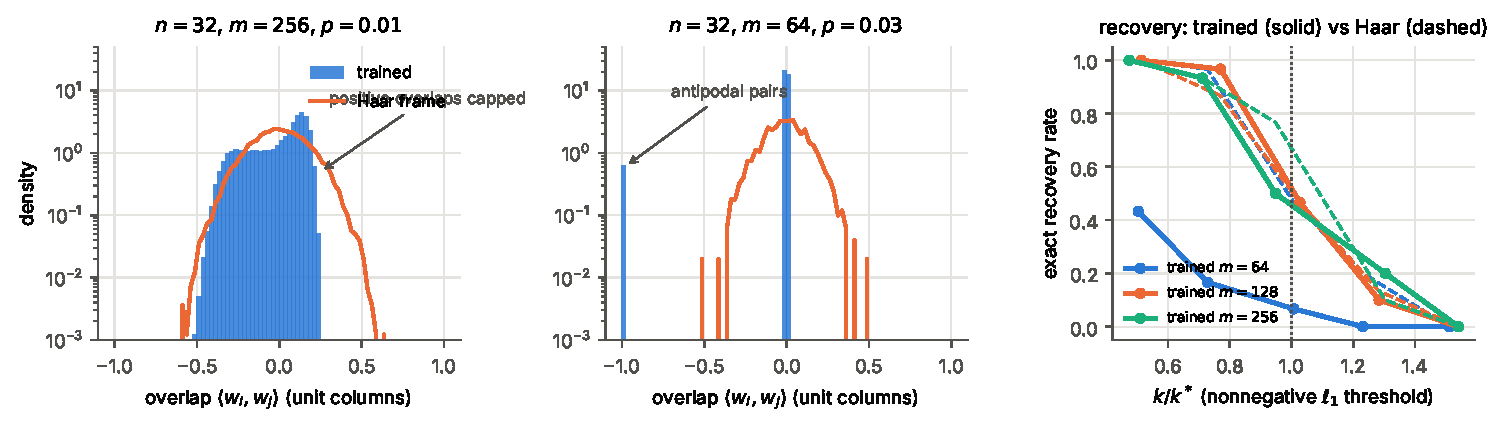
\includegraphics[width=\linewidth]{figs/e02_tms.pdf}
\caption{E02. Left: overlaps between trained feature directions (bars) and between Haar-frame directions (line)
for $m=256$, $p=0.01$; trained codes are platykurtic, with fewer large overlaps. Middle: $m=64$; the trained code is
32 antipodal pairs. Right: exact recovery of nonnegative $k$-sparse combinations by $\ell_1$ minimization, trained
vs Haar, with the predicted threshold $k^*$ (dashed).}
\label{fig:e02}
\end{figure}
Three findings. (i) Every trained code is an essentially exact tight frame, so by \cref{prop:frame-identity} its
second moment \emph{must} match Haar; it does, to three digits. (ii) Beyond second order the trained codes are not
Haar. With $m=2n$ they are $n$ antipodal pairs---excess kurtosis $\approx60$, coherence $1$---a highly structured
code that is ideal for nonnegative features and a ReLU readout and terrible for signed ones. With $m=8n$ they are
\emph{better} than Haar at the extremes: negative excess kurtosis and lower coherence. Training finds structured
codes, as engineers do; the random code is the floor. (iii) On the task they were trained for, trained codes beat
the best uniformly-biased Haar frame by large factors, yet their $\ell_1$ recovery thresholds are close to the
Haar threshold and to the statistical-dimension prediction, consistent with the universality of that
threshold~\cite{Monajemi}.

\subsection{E03: language-model embeddings}
We extracted the RoBERTa-base~\cite{RoBERTa} token embedding matrix ($m=50{,}261$ tokens, $n=768$) and GloVe
100d~\cite{GloVe} ($m=400{,}000$, $n=100$) and treated vocabulary items as features. Each is analysed raw, centred
(mean removed) and whitened (multiplied by $\Sigma^{-1/2}$, which forces a tight frame) (\cref{tab:e03},
\cref{fig:e03}).
\begin{table}[h]\centering\footnotesize
\resizebox{\linewidth}{!}{\begin{tabular}{@{}ll cc c cc cc c@{}}\toprule
 & & $n\,\E\cos^2$ & excess & & \multicolumn{2}{c}{$\Pr(|\cos|>t)$} & \multicolumn{2}{c}{max coherence} & tight- \\
model & version & (Haar $\approx1$) & kurt. & $t$ & observed & Gaussian & observed & Haar & ness \\\midrule
RoBERTa & raw & 2.70 & 2.77 & 0.2 & 4.9e-03 & 3.0e-08 & 0.81 & 0.17 & 0.35 \\
 & centred & 2.13 & 3.05 & 0.2 & 2.5e-03 & 3.0e-08 & 0.81 & 0.17 & 0.43 \\
 & whitened & 0.99 & 5.09 & 0.2 & 2.9e-04 & 3.0e-08 & 0.88 & 0.17 & 0.85 \\
\addlinespace
GloVe & raw & 4.77 & -0.26 & 0.5 & 1.7e-02 & 5.7e-07 & 0.96 & 0.55 & 0.20 \\
 & centred & 1.53 & 0.64 & 0.5 & 9.1e-04 & 5.7e-07 & 0.98 & 0.55 & 0.65 \\
 & whitened & 1.02 & 0.42 & 0.5 & 2.0e-04 & 5.7e-07 & 0.94 & 0.55 & 0.96 \\
\bottomrule\end{tabular}}

\medskip
\resizebox{0.6\linewidth}{!}{\begin{tabular}{@{}lrr ccc@{}}\toprule
 & & & \multicolumn{3}{c}{exact $\ell_1$ recovery rate} \\
model & $m_{\rm sub}$ & $k$ ($k^*$) & centred & whitened & Haar \\\midrule
RoBERTa & 1536 & 222 (296) & 1.00 & 1.00 & 1.00 \\
RoBERTa & 1536 & 296 (296) & 0.50 & 0.50 & 0.62 \\
RoBERTa & 1536 & 370 (296) & 0.00 & 0.00 & 0.00 \\
GloVe & 200 & 19 (39) & 1.00 & 1.00 & 1.00 \\
GloVe & 200 & 29 (39) & 1.00 & 1.00 & 0.97 \\
GloVe & 200 & 35 (39) & 0.83 & 0.93 & 0.83 \\
GloVe & 200 & 39 (39) & 0.57 & 0.47 & 0.43 \\
GloVe & 200 & 42 (39) & 0.23 & 0.27 & 0.30 \\
GloVe & 200 & 48 (39) & 0.00 & 0.00 & 0.03 \\
\bottomrule\end{tabular}}
\caption{E03: language-model embeddings as codes. Top: overlap statistics over $4\times10^5$ random pairs; $t$ is the tabulated threshold nearest $4/\sqrt n$ ($5.5/\sqrt n$ for RoBERTa, $5/\sqrt n$ for GloVe);
the Gaussian column is the tail of $\mathcal N(0,1/n)$; coherence over 4000 random items. Bottom: signed $\ell_1$
recovery from a random sub-dictionary of $m_{\rm sub}=2n$ items ($k^*$: predicted threshold; RoBERTa 8 trials per
entry, GloVe 30).}
\label{tab:e03}\end{table}

\begin{figure}[t]
\centering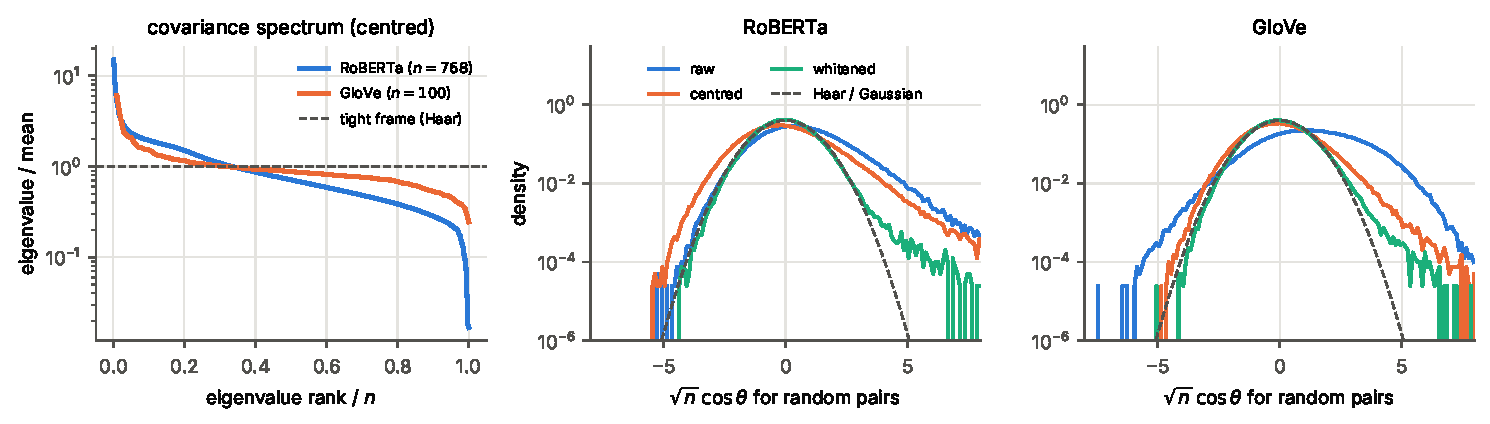
\includegraphics[width=\linewidth]{figs/e03_embeddings.pdf}
\caption{E03. Left: covariance spectra of centred embeddings, normalized to mean one; a Haar (tight) frame is the
flat line. Middle and right: distribution of $\sqrt n\cos\theta$ for random pairs, raw, centred and whitened, against
the Haar/Gaussian prediction (dashed). Whitening restores the bulk; the tails remain heavy.}
\label{fig:e03}
\end{figure}
Real embeddings depart from Haar in two layers. The first is \emph{anisotropy}: a common mean direction and a
spectrum far from flat, so the frame is far from tight and the mean-square overlap is several times the Haar value
(a known property of language-model embeddings~\cite{Ethayarajh}). Whitening removes this by construction and
returns the second moment to $1/n$ (again by \cref{prop:frame-identity}). The second layer survives whitening: the
\emph{tails} of the overlap distribution are far heavier than Gaussian. Listing the most coherent pairs
(\file{scripts/e03\_top\_pairs.py}) shows what they are. In RoBERTa they are the same word with and without a
leading space or capital (``As''/``\,As'', ``Georgia''/``\,Georgia'', ``Education''/``education''), inflections
(``turned''/``turning'', ``tend''/``tends'') and near-synonyms (``spokesman''/``spokeswoman'',
``Usually''/``Normally''), with $\abs{\cos}\approx0.7$--$0.9$. In GloVe they are rare tokens of one type: numbers
(``28.6''/``24.9'', ``1679''/``1677'', ``84-year''/``83-year''), Polish place names, moth genera. Either way they
are not independent features at all. Nevertheless the bulk
behaves like a random code: $\ell_1$ recovery of random sparse combinations from a random sub-dictionary with $m=2n$
sits at the Haar threshold.

Two cautions keep this last result in proportion. First, it is less surprising than it looks: the Donoho--Tanner
transition is known to be universal well beyond Gaussian matrices, including for many deterministic
frames~\cite{Monajemi}, and we are seeing one more instance. Second, our test draws random supports, which is the
typical case where agreement is expected. Real activations co-activate correlated features (the near-duplicates
above), and a random-support test cannot see that. The embeddings tested are input embeddings; dictionaries of
internal representations (sparse autoencoders on a residual stream) are the test that matters most and were not
reachable here.

\subsection{What this means for the correspondence}\label{sec:part1-meaning}
The Haar code is the right null model and the wrong description. Statements about \emph{typical} sparse sets
(recovery thresholds, the restricted isometry of random supports) transfer from Haar codes to trained ones,
because they depend on second-order structure, which tight frames share. Statements about \emph{worst-case} sets
(coherence, the cheapest null vector) do not: trained codes can be better than random (toy models with plentiful
features) or much worse (embeddings with near-duplicates). In black hole language, a trained code is a designed
error-correcting code rather than a scrambler's typical one---which raises the question, not pursued here, of
whether a black hole's actual code (as opposed to its Haar model) has analogous structure.


\part*{Part II.\quad Legibility and accidental obfuscation}
% ============================================================== PART II
\section{Setting: a channel, a public frame, and monitors}\label{sec:setting}

Part~I was about the \emph{geometry} of a code: its Gram matrix, which is invariant under rotations of the
fundamental space. Monitoring depends on the part of the code that is \emph{not} rotation invariant: how its
features sit relative to a frame that an outside observer knows. Natural language is such a frame, and so is a
sparse-autoencoder dictionary or the neuron basis. When two models communicate in activations rather than tokens
(latent reasoning~\cite{Coconut}, activation handoff between agents), the question is whether training keeps the
message legible in the frame the overseer reads.

\begin{figure}[h]
\centering\ChannelPicture
\caption{The toy model of Part II. A sender writes a message $h$ in $\R^n$; the public frame is the coordinate
basis, made meaningful by the coordinatewise nonlinearity. The receiver reads a noisy copy. A linear monitor reads
$h$, either frozen at a legible checkpoint, recalibrated, or refit.}
\label{fig:channel}
\end{figure}

\subsection{The model}
Features $x\in\{0,1\}^d$ are i.i.d.\ Bernoulli($p$). The sender writes $h=\tanh(Ax+a)\in\R^n$; the channel adds
$\sigma\xi$ with $\xi\sim\mathcal N(0,I)$; a one-hidden-layer receiver outputs logits for $x$; the loss is the
summed binary cross-entropy. Unless stated otherwise $n=16$, $\sigma=0.1$, $p=0.1$, the receiver has 64 hidden
units, and training uses minibatches of 256. A code is \emph{legible} if each feature drives one public coordinate:
$A_{jl}=0$ unless $j=o(l)$, the coordinate it owns. We produce legible codes by training with an $\ell_1$ budget
$\lambda\sum_j\abs{h_j}$ in the public frame, and then ask what happens when training continues.

\subsection{What we measure}
Two kinds of legibility, which turn out to behave differently.
\begin{itemize}[leftmargin=*]
\item \emph{Feature-level spread}: the participation ratio of each sender column, $\big(\sum_jA_{jl}^2\big)^2/\sum_jA_{jl}^4$,
averaged over features (``neurons per feature''; 1 for a legible code).
\item \emph{Monitor-level legibility}: the F1 score of linear monitors reading $h$. The \emph{frozen} monitor is a
logistic probe fit at the legible checkpoint and never touched again. The \emph{recalibrated} monitor keeps the
frozen directions and refits only a scale and bias per feature. The \emph{refit} monitor is retrained on the
current code with the same budget as the frozen one. The receiver's own F1 bounds what is in the channel.
\end{itemize}
The differences between consecutive levels in \cref{fig:ladder} separate three effects that earlier drafts of these
notes conflated.

\begin{figure}[h]
\centering\MonitorLadder
\caption{Four readings of the same message. Frozen $\to$ recalibrated measures calibration drift (amplitudes and
offsets changed; cheap to repair with labels). Recalibrated $\to$ refit measures frame drift (the directions
changed). Refit $\to$ receiver measures information the receiver uses that no linear public decoder recovers.}
\label{fig:ladder}
\end{figure}

\section{Theory: the legible critical point}\label{sec:saddle}

\subsection{What privileges the public frame}
\begin{proposition}\proved
If the sender were linear, $h=Ax$, with an $\ell_2$ power constraint, then for every orthogonal $O$ the codes $A$
and $OA$ achieve the same optimal loss (the receiver absorbs $O^\top$, and the noise is isotropic). There is no
preferred frame, and ``legible'' is not a meaningful property.
\end{proposition}
The coordinatewise $\tanh$ breaks this symmetry, because it bounds each coordinate separately. This is the
``privileged basis'' of~\cite{TMS}, and it has a second consequence. The feasible set of messages is a cube, and a
message that uses $k$ coordinates has energy at most $k$, whereas one that uses all $n$ coordinates can have energy
$n$ while still respecting each bound. Against isotropic noise, energy buys distinguishability. So the same feature of the
architecture that makes the public frame meaningful also makes spreading across it pay. (An earlier draft argued
that spreading pays from energy considerations alone; without the per-coordinate bound that argument is false,
since rotating a code changes nothing.)

\subsection{Stationarity in leak directions}
\begin{lemma}\label{lem:stationary}\proved
Let the code be legible and let $j$ be an \emph{empty} coordinate (owned by no feature), so $h_j=\tanh(a_j)$ is
constant. If the receiver ignores $j$ ($B_{:,j}=0$), then $\partial L/\partial A_{jl}=0$ and
$\partial^2L/\partial A_{jl}^2=0$ for every feature $l$.
\end{lemma}
\begin{proof}
$\partial L/\partial A_{jl}=\E\big[(\sum_u\delta_uB_{uj})\,\phi'(z_j)\,x_l\big]$ with $\delta=\partial L/\partial v$,
which vanishes when $B_{:,j}=0$. Differentiating again, every term carries a factor of $B_{:,j}$.
\end{proof}
At the receiver's optimum, reading a coordinate that carries only noise does not help, so one expects
$B_{:,j}\approx0$. (Trained receivers do not get there, because the cost of reading noise is second order and
suppressed by the receiver's confidence. In practice the lemma holds in the weaker form that the leak gradient is
proportional to $B_{:,j}$ times the residual error; see E13.) Leaks into a coordinate \emph{owned by another feature} have no such protection. With more features
than coordinates (superposition) every coordinate is owned, and a legible code need not be a critical point at all.

\subsection{Envelope curvature: the I-MMSE formula}
If the receiver re-optimizes as the sender leaks, the relevant quantity is the curvature of the envelope.
\begin{proposition}[Envelope curvature]\label{prop:immse}\proved\ (for the Bayes receiver)
Let $\ell$ own coordinate $o(\ell)$ and leak by $\varepsilon$ into empty coordinate $j$, and let the receiver be
Bayes-optimal. Then
\[
\frac{d^2L_{\rm env}}{d\varepsilon^2}\Big|_{\varepsilon=0}=-\frac{\phi'(a_j)^2\,\mmse_\ell}{\sigma^2},
\]
where $\mmse_\ell=\E(x_\ell-\E[x_\ell\mid y])^2$ is the residual error of feature $\ell$ and $\phi'=1-\tanh^2$.
\end{proposition}
\begin{proof}
Features are independent and each coordinate depends on one feature, so the loss for $\ell$ is
$H(x_\ell)-I(x_\ell;y)$. The leak adds a second Gaussian observation of $x_\ell$ with gap $\phi'(a_j)\varepsilon$ and
noise $\sigma$; the two observations combine into one with $\mathrm{snr}=(g_\ell^2+\phi'(a_j)^2\varepsilon^2)/\sigma^2$.
By the I-MMSE relation~\cite{GSV}, $dI/d\,\mathrm{snr}=\frac12\mmse$ for any input distribution, so
$d^2I/d\varepsilon^2|_0=\phi'(a_j)^2\mmse_\ell/\sigma^2$.
\end{proof}
The formula unifies two sources of negative curvature that earlier drafts treated separately. When a feature is read
poorly because of interference, $\mmse_\ell$ stays large and the force is $\propto1/\sigma^2$. When it is read poorly
because of noise, $\mmse_\ell$ is a Gaussian tail and the force is non-monotone in $\sigma$.

\subsection{What gradient descent actually sees: the handshake}
Gradient descent follows the joint Hessian, not the envelope. Restricted to the leak $\varepsilon=A_{j\ell}$ and the
read $r=B_{:,j}$, \cref{lem:stationary} gives the block
\[
\mathcal H=\begin{pmatrix}0&C^\top\\ C&H_{rr}\end{pmatrix},\qquad
\lambda_-=\tfrac12\Big(h-\sqrt{h^2+4\norm C^2}\Big)\approx-\norm C\quad(h\ll\norm C),
\]
with $h$ the receiver curvature along $C$ \heur. The sender cannot profit from leaking until the receiver reads,
and the receiver cannot profit from reading until the sender leaks: the unstable direction is half leak, half read,
and the envelope curvature is the Schur complement $-C^\top H_{rr}^{-1}C$. Under gradient descent with step $\eta$,
a perturbation of size $z_0$ escapes in a time of order $\log(1/z_0)/(\eta\abs{\lambda_-})$, so a code whose features
are already well read lingers at the saddle. Note what this implies at the extreme: every curvature in this picture
carries a factor of the receiver's residual error (\cref{prop:immse}), so when the features are decoded almost
perfectly the saddle is almost flat, and gradient descent does not leave it at all on any practical time scale.

Adam divides each coordinate's update by a running estimate of its gradient magnitude. Near the saddle that
magnitude is tiny, and the normalized step has size $\approx\eta$ regardless of $\norm C$. Two consequences follow:
\begin{enumerate}[leftmargin=*]
\item Adam's escape time is essentially independent of the curvature (\cref{fig:handshake}).
\item Even where the expected gradient vanishes, minibatch noise in the leak gradient is normalized into
steps of size $\sim\eta$. So the sender random-walks off the legible support whether or not the receiver reads the
result. The message densifies without being used.
\end{enumerate}
The second mechanism needs no negative curvature at all. E13 below finds that it is the one operating at the noise
level of our drift experiments, where the legible point is flat to numerical precision.

\begin{prediction}\label{pred:writer}
Spread of the message in the public frame is controlled by the update rule of the parameters that \emph{write} the
message. Plain SGD on the sender preserves legibility even if everything else uses Adam; Adam on the sender spreads
the message even if the receiver uses SGD.
\end{prediction}

\begin{figure}[t]
\centering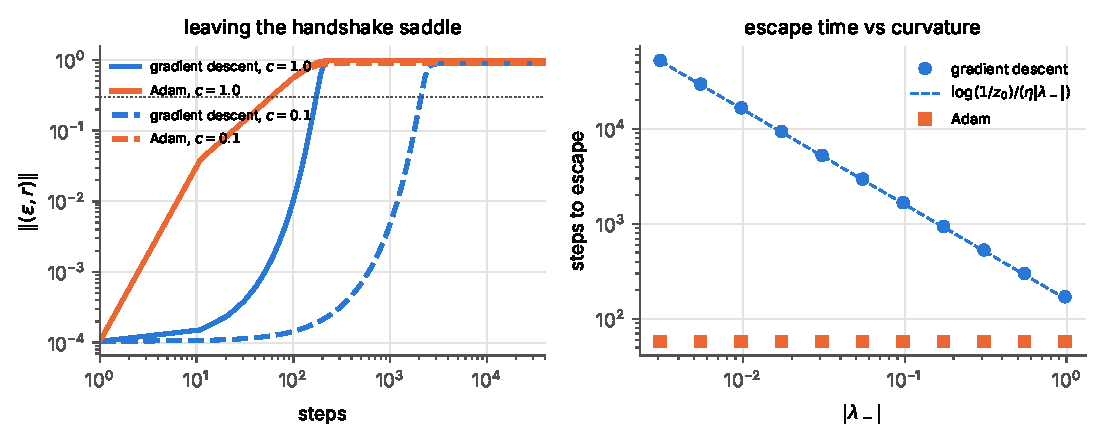
\includegraphics[width=0.85\linewidth]{figs/e14_handshake.pdf}
\caption{E14: the handshake saddle in isolation, $L=c\,\varepsilon r+\frac h2r^2+\frac q4(\varepsilon^2+r^2)^2$ with
$h=0.05c$, $q=c$. Left: distance from the saddle against steps; gradient descent waits, then grows exponentially;
Adam (both values of $c$ coincide) leaves at once. Right: escape time against $\abs{\lambda_-}$ over two and a half
decades. Gradient descent takes 1.6--4\% longer than $\log(1/z_0)/(\eta\abs{\lambda_-})$ (the excess grows with
$\abs{\lambda_-}$, where the discrete-step and quartic corrections matter); Adam takes 58 steps throughout.}
\label{fig:handshake}
\end{figure}

\section{Experiments: drift, optimizers, and the saddle}\label{sec:part2-exp}

\subsection{E10: what happens to a legible code}
Starting from a legible code with $d=32$ features in $n=16$ coordinates, we continue training under Adam in four
ways (\cref{tab:e10}, \cref{fig:e10}).
\begin{table}[h]\centering\footnotesize
\resizebox{\linewidth}{!}{\begin{tabular}{@{}l ccccc@{}}\toprule
condition (after 6000 steps) & receiver F1 & frozen & recalibrated & refit & neurons/feature \\\midrule
legible checkpoint & 0.915\,$\pm$\,0.018 & 0.922\,$\pm$\,0.019 & 0.927\,$\pm$\,0.015 & 0.922\,$\pm$\,0.017 & 1.159\,$\pm$\,0.123 \\\midrule
release & 0.984\,$\pm$\,0.001 & 0.714\,$\pm$\,0.047 & 0.865\,$\pm$\,0.061 & 0.937\,$\pm$\,0.013 & 1.733\,$\pm$\,0.336 \\
pressure & 0.922\,$\pm$\,0.006 & 0.790\,$\pm$\,0.066 & 0.839\,$\pm$\,0.053 & 0.893\,$\pm$\,0.015 & 1.085\,$\pm$\,0.055 \\
pressure+budget & 0.827\,$\pm$\,0.012 & 0.772\,$\pm$\,0.052 & 0.798\,$\pm$\,0.026 & 0.822\,$\pm$\,0.021 & 1.214\,$\pm$\,0.216 \\
pressure+monitor & 0.907\,$\pm$\,0.004 & 0.803\,$\pm$\,0.018 & 0.872\,$\pm$\,0.030 & 0.870\,$\pm$\,0.011 & 1.241\,$\pm$\,0.156 \\
\bottomrule\end{tabular}}
\caption{E10: four continuations of a legible code ($d=32$, $n=16$, Adam), mean $\pm$ sd over 5 seeds. ``pressure'':
feature density $p$ raised from 0.1 to 0.3; ``budget'': the $\ell_1$ legibility budget is kept; ``monitor'': the
frozen monitor's loss is added to the training loss. Receiver$-$refit gap: 0.029\,$\pm$\,0.019 under pressure, 0.037\,$\pm$\,0.011 with the monitor in the loss.}
\label{tab:e10}\end{table}

\begin{figure}[h]
\centering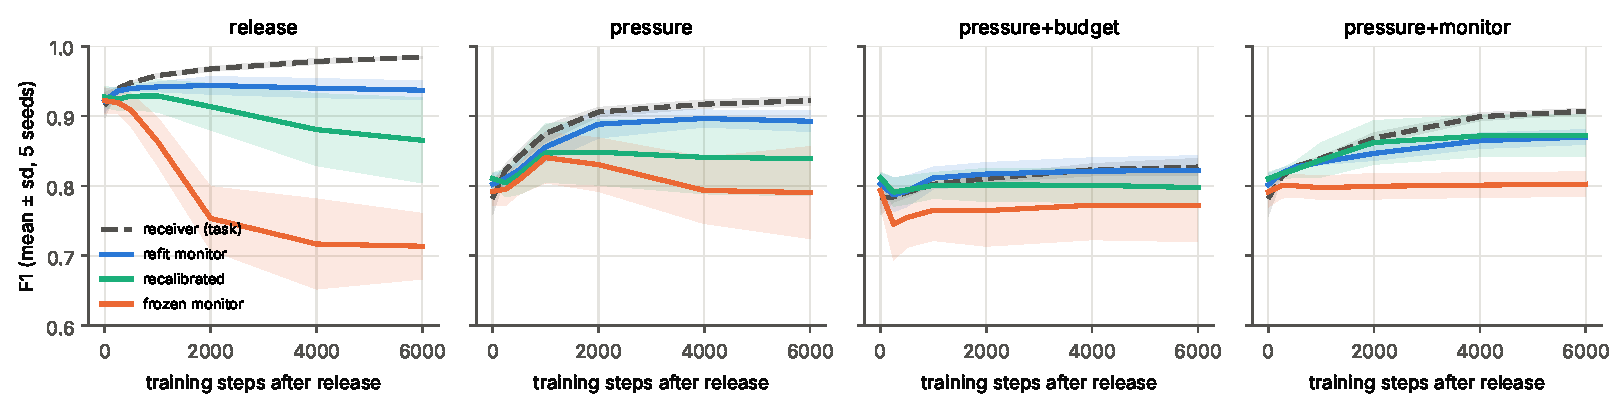
\includegraphics[width=\linewidth]{figs/e10_drift.pdf}
\caption{E10: the four readings of \cref{fig:ladder} over training, mean $\pm$ sd over 5 seeds.}
\label{fig:e10}
\end{figure}

\emph{Release} (the budget is removed and nothing else changes) is the cleanest case. The code spreads: neurons per
feature rise from $1.16$ to $1.73$. The frozen monitor falls from $0.92$ to $0.71$. But a per-feature recalibration
of scale and bias recovers most of that ($0.87$), and a refit monitor reads the new code as well as the old ($0.94$).
The honest decomposition of the frozen monitor's loss is roughly two-thirds calibration and one-third direction.
Neither is invisible: a monitor that is refit, or even just recalibrated, on fresh labelled data sees through it.

\emph{Pressure} (three times as many active features) does not spread the code at the feature level; neurons per
feature fall slightly. \emph{Pressure with the budget kept} holds the code legible at a visible price in task
performance (receiver F1 $0.83$ against $0.92$): the legibility tax. \emph{Pressure with the frozen monitor in the
loss} does what one would expect of a training signal: the frozen monitor's score stops falling. The worry from
earlier drafts was that the receiver would meanwhile build a channel no monitor can read. At this scale we see no
sign of it: the receiver$-$refit gap is the same with and without the monitor in the loss, within seed-to-seed
variation.

\subsection{E11: the update rule}
We now hold the task fixed, remove the budget, and change only the update rule (\cref{tab:e11},
\cref{fig:e11}).
\begin{table}[h]\centering\footnotesize\setlength{\tabcolsep}{3pt}
\resizebox{\linewidth}{!}{\begin{tabular}{@{}l cccccc@{}}\toprule
optimizer (6000 steps, budget removed) & receiver F1 & frozen & recalibrated & refit & neurons/feature & leak \\\midrule
$d=12$, legible start & 0.985\,$\pm$\,0.003 & 0.998\,$\pm$\,0.004 & 0.998\,$\pm$\,0.004 & 0.998\,$\pm$\,0.004 & 1.033\,$\pm$\,0.066 & 0.013\,$\pm$\,0.026 \\
\quad Adam & 1.000\,$\pm$\,0.000 & 0.998\,$\pm$\,0.004 & 0.998\,$\pm$\,0.004 & 1.000\,$\pm$\,0.000 & 2.066\,$\pm$\,0.097 & 0.330\,$\pm$\,0.016 \\
\quad SGD & 1.000\,$\pm$\,0.000 & 0.998\,$\pm$\,0.003 & 0.998\,$\pm$\,0.003 & 1.000\,$\pm$\,0.000 & 1.107\,$\pm$\,0.132 & 0.045\,$\pm$\,0.052 \\
\quad hybrid: SGD sender, Adam receiver & 1.000\,$\pm$\,0.000 & 0.998\,$\pm$\,0.003 & 0.998\,$\pm$\,0.003 & 1.000\,$\pm$\,0.000 & 1.078\,$\pm$\,0.094 & 0.032\,$\pm$\,0.038 \\
\quad reverse: Adam sender, SGD receiver & 1.000\,$\pm$\,0.000 & 0.998\,$\pm$\,0.004 & 0.998\,$\pm$\,0.004 & 1.000\,$\pm$\,0.000 & 1.726\,$\pm$\,0.215 & 0.315\,$\pm$\,0.172 \\
\quad SGD, large step & 0.856\,$\pm$\,0.201 & 0.430\,$\pm$\,0.142 & 0.516\,$\pm$\,0.202 & 0.843\,$\pm$\,0.211 & 3.884\,$\pm$\,0.545 & 0.620\,$\pm$\,0.164 \\
\midrule
$d=32$, legible start & 0.916\,$\pm$\,0.017 & 0.927\,$\pm$\,0.022 & 0.934\,$\pm$\,0.020 & 0.926\,$\pm$\,0.021 & 1.269\,$\pm$\,0.172 & 0.071\,$\pm$\,0.028 \\
\quad Adam & 0.982\,$\pm$\,0.002 & 0.708\,$\pm$\,0.052 & 0.867\,$\pm$\,0.070 & 0.941\,$\pm$\,0.015 & 1.775\,$\pm$\,0.432 & 0.069\,$\pm$\,0.030 \\
\quad SGD & 0.960\,$\pm$\,0.004 & 0.796\,$\pm$\,0.083 & 0.919\,$\pm$\,0.039 & 0.943\,$\pm$\,0.014 & 1.561\,$\pm$\,0.350 & 0.102\,$\pm$\,0.048 \\
\quad hybrid: SGD sender, Adam receiver & 0.982\,$\pm$\,0.002 & 0.760\,$\pm$\,0.050 & 0.886\,$\pm$\,0.055 & 0.944\,$\pm$\,0.015 & 1.765\,$\pm$\,0.401 & 0.098\,$\pm$\,0.037 \\
\quad reverse: Adam sender, SGD receiver & 0.962\,$\pm$\,0.003 & 0.769\,$\pm$\,0.081 & 0.916\,$\pm$\,0.040 & 0.944\,$\pm$\,0.013 & 1.547\,$\pm$\,0.367 & 0.065\,$\pm$\,0.033 \\
\quad SGD, large step & 0.426\,$\pm$\,0.357 & 0.232\,$\pm$\,0.045 & 0.143\,$\pm$\,0.195 & 0.426\,$\pm$\,0.301 & 2.361\,$\pm$\,0.842 & 0.687\,$\pm$\,0.208 \\
\bottomrule\end{tabular}}
\caption{E11: same task, legibility budget removed, five update rules; mean $\pm$ sd over 5 seeds. Learning rates:
Adam $3\times10^{-3}$, SGD $0.05$, large-step SGD $0.5$. ``leak'': fraction of sender weight energy outside each
feature's legible coordinate. $d=12<n$: empty coordinates exist; $d=32>n$: superposition.}
\label{tab:e11}\end{table}

\begin{figure}[h]
\centering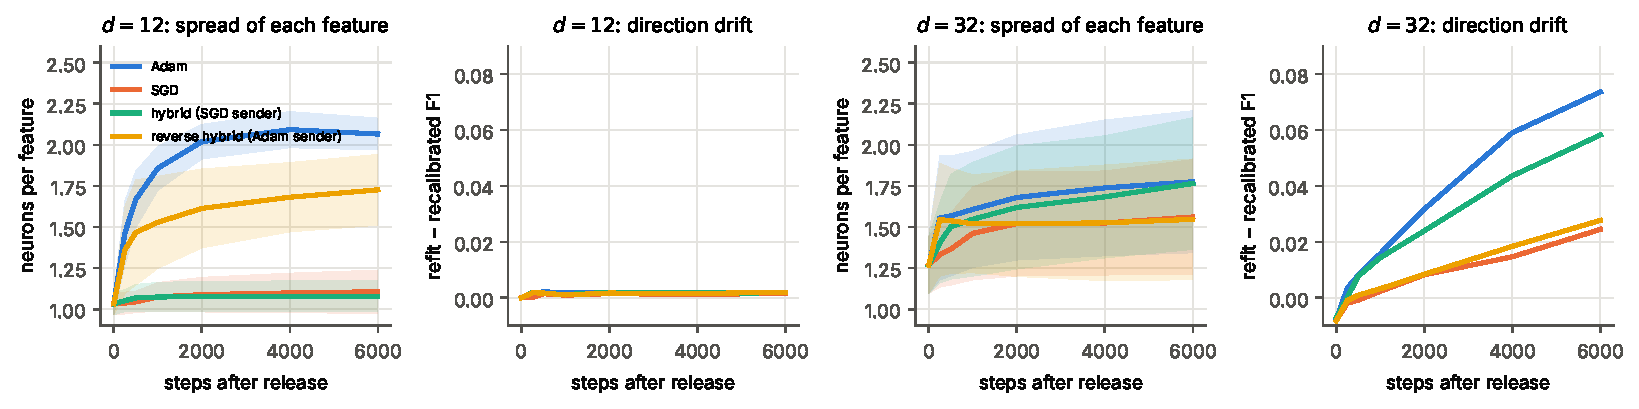
\includegraphics[width=\linewidth]{figs/e11_optimizers.pdf}
\caption{E11: feature spread and direction drift (refit minus recalibrated F1) after the budget is removed, for four
update rules, mean $\pm$ sd over 5 seeds. Large-step SGD diverges on some seeds and is shown only in \cref{tab:e11}.}
\label{fig:e11}
\end{figure}

\emph{With spare public coordinates ($d=12<n$), \cref{pred:writer} holds.} At identical task performance (F1 $1.000$
for all four rules), the sender's update rule decides whether features stay on their coordinates. Adam on the sender
spreads each feature over about two neurons, whether the receiver uses Adam ($2.07$) or SGD ($1.73$). SGD on the
sender keeps it on one ($1.11$ with SGD everywhere, $1.08$ for the hybrid with an Adam receiver). This is the
hybrid optimizer of earlier drafts, and in this regime it works as advertised. The spread is also exactly the kind
predicted by \cref{sec:saddle}: under Adam on the sender, the message densifies even when the receiver (on SGD) is
too slow to make use of it. In this regime the spread does not hurt linear monitors, which remain at $0.998$ in
every column: the new copies are redundant, and the original coordinate still carries each feature.

\emph{In superposition ($d=32>n$), \cref{pred:writer} fails.} E11's starting codes differ in how they are packed
(\file{e11\_packing.py}): at $d=12$, 11 or 12 of the 16 coordinates are used and at most one is shared; at $d=32$,
10 to 16 coordinates are shared by 2--4 features each, and at most two are empty. So \cref{lem:stationary} has
almost nothing to protect, and E15 below shows that leaks into occupied coordinates feel first-order forces. Spread and direction
drift now track the \emph{receiver's} update rule: with an Adam receiver (Adam everywhere, or the hybrid) neurons per
feature reach $1.77$ and direction drift is $0.06$--$0.07$; with an SGD receiver (SGD everywhere, or the reverse
hybrid) they are $1.55$ and $0.02$--$0.03$. These are also the configurations whose receivers learn more (task F1
$0.982$ against $0.960$). The natural reading is that, in superposition, drift away from the public frame is
a first-order response to a receiver that is still improving, and the optimizer matters through how fast the
receiver improves rather than through the sender's normalization. The hybrid optimizer does not preserve legibility
here at matched task performance.

\subsection{E15: superposition removes the critical point}
Is the legible code a critical point when coordinates are shared? We take E11's starting codes (same seeds, same
ReLU receiver), restrict each feature to its strongest coordinate while keeping whatever sharing the code had, polish
all parameters within that support on a full batch, and then measure the gradient in the directions that leave it
(\cref{tab:e15}).
\begin{table}[h]\centering\footnotesize\setlength{\tabcolsep}{3pt}
\resizebox{\linewidth}{!}{\begin{tabular}{@{}rr cc cc cc c@{}}\toprule
 & & \multicolumn{2}{c}{coordinates (of 16)} & \multicolumn{2}{c}{gradient within support} & \multicolumn{2}{c}{gradient, leaks into occupied} & leaks into \\\cmidrule(lr){3-4}\cmidrule(lr){5-6}\cmidrule(lr){7-8}
$d$ & seeds & empty & shared & norm & per entry & norm & per entry & empty, norm \\\midrule
12 & 3 & 4.3 & 0.3 & 1.9e-09--2.7e-07 & 4.3e-11--6.1e-09 & 7.7e-10--6.6e-07 & 6.4e-11--5.7e-08 & 2.7e-10--2.7e-07 \\
32 & 3 & 0.3 & 13.7 & 2.9e-02--4.1e-02 & 5.1e-04--7.3e-04 & 1.5e-01--1.8e-01 & 7.0e-03--8.1e-03 & 0.0e+00--3.9e-04 \\
\bottomrule\end{tabular}}
\caption{E15: is the legible code a critical point? Starting from E11's legible codes (same seeds, ReLU receiver), each
feature is restricted to its strongest coordinate (shared coordinates kept) and all parameters are polished within that
support (full batch of 6144, $\sigma=0.1$). Gradient norms, and root-mean-square per entry, in three groups of
directions; ranges are over seeds.}
\label{tab:e15}\end{table}

At $d=12$ the polish converges, and the legible code is a critical point in every direction, leaks included:
all gradient norms lie between $10^{-9}$ and $10^{-6}$. At $d=32$ it is not. After the same 11{,}000 full-batch steps the gradient
within the legible support is still $3$--$4\times10^{-2}$, and the gradient for leaks into occupied coordinates is
$0.15$--$0.18$ in norm, 11--14 times larger per entry. In superposition the legible support is not where the loss
wants to be. Drift away from it is a first-order response, which any optimizer will follow, and which makes the
update rule matter mainly through how fast the receiver keeps improving. That is the pattern E11 shows.

\subsection{E13: how flat is the legible critical point?}
To look for the saddle of \cref{sec:saddle} directly we use $d=12$ features (so empty coordinates exist), a smooth
softplus receiver (so second derivatives exist), and channel noise from the operating value $\sigma=0.1$ up to
$\sigma=0.9$. We match each feature to its own coordinate, restrict the sender to that legible support, and polish
everything to a critical point within it, on a fixed batch of 6144 samples. We then compute the global smallest
Hessian eigenvalue by Lanczos and, for the least saturated empty coordinate, the leak/read block of each feature
(\cref{tab:e13}, \cref{fig:e13}).
\begin{table}[h]\centering\footnotesize\setlength{\tabcolsep}{3pt}
\resizebox{\linewidth}{!}{\begin{tabular}{@{}c c cc cc cc ccc@{}}\toprule
 & sender & \multicolumn{2}{c}{residual error $\mmse$} & \multicolumn{2}{c}{gradient norm} & \multicolumn{2}{c}{global $\lambda_{\min}$} & \multicolumn{3}{c}{leak into empty coordinate (median over features)} \\\cmidrule(lr){3-4}\cmidrule(lr){5-6}\cmidrule(lr){7-8}\cmidrule(l){9-11}
$\sigma$ & gap & batch & fresh noise & within & leak, empty & value & on leak & $H_{\varepsilon\varepsilon}$ (lemma: 0) & envelope & I-MMSE \\\midrule
0.1 & 1.27 & 4e-18 & 3e-11 & 6e-09 & 4e-10 & -5e-10 & 0.04 & 1e-10 & 1e-10 & -6e-13 \\
0.2 & 1.61 & 2e-17 & 4e-05 & 7e-09 & 1e-09 & -1e-09 & 0.69 & 8e-10 & 4e-10 & -8e-05 \\
0.4 & 1.97 & 7e-14 & 8e-03 & 1e-07 & 9e-08 & -6e-08 & 0.38 & 3e-07 & 2e-07 & -2e-03 \\
0.6 & 2.00 & 1e-02 & 3e-02 & 1e-03 & 2e-02 & -8e-04 & 0.07 & 1e-01 & 1e-01 & -5e-02 \\
0.9 & 2.00 & 4e-02 & 6e-02 & 2e-03 & 2e-02 & -2e-02 & 0.85 & 5e-02 & 1e-02 & -6e-02 \\
\bottomrule\end{tabular}}
\caption{E13: the legible critical point ($d=12$, $n=16$, softplus receiver), polished on a fixed batch of
6144 samples with fixed channel noise. Sender gap: $|\tanh(A_{o\ell}+a_o)-\tanh(a_o)|$, at most 2.
Residual error of the trained receiver on that batch and on fresh noise (\file{e13\_fresh.py}). Gradient norm within the
legible subspace and for leaks into empty coordinates. Global $\lambda_{\min}$ by Lanczos and the weight of its
eigenvector on leaks into empty coordinates. Last three columns: for the least saturated empty coordinate, the leak
curvature $H_{\varepsilon\varepsilon}$, the envelope (Schur-complement) curvature, and the I-MMSE prediction
$-\phi'(a_j)^2\mmse_\ell/\sigma^2$ of \cref{prop:immse} with the fresh-noise error.}
\label{tab:e13}\end{table}

\begin{figure}[h]
\centering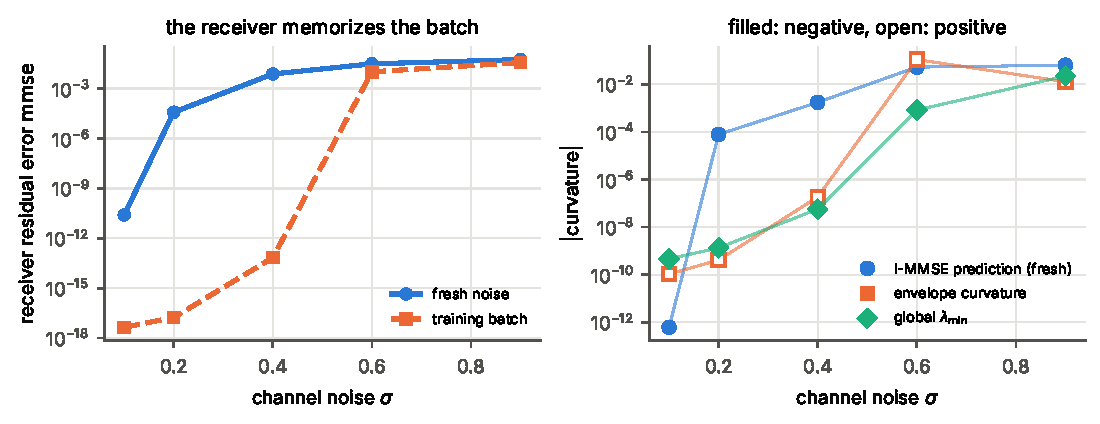
\includegraphics[width=0.9\linewidth]{figs/e13_saddle.pdf}
\caption{E13. Left: residual error of the polished receiver on its training batch and on fresh channel noise; for
$\sigma\le0.4$ the receiver has memorized the noise in its batch. Right: magnitudes of the I-MMSE prediction (with the
fresh-noise error), of the measured envelope curvature (median over features), and of the global smallest Hessian
eigenvalue; filled markers are negative, open markers positive.}
\label{fig:e13}
\end{figure}
Three findings, one of them negative.

\emph{At the operating point the legible code is flat, not a saddle.} At $\sigma=0.1$, the noise level of E10 and
E11, the polished point is critical to $6\times10^{-9}$, and the global $\lambda_{\min}$, the leak curvatures and the
envelope curvatures are all below $10^{-9}$ in magnitude. This is not an artefact. The
receiver's error on fresh noise is itself a few times $10^{-11}$, so \cref{prop:immse} predicts a negative curvature of
order $10^{-12}$. Every second derivative of the cross-entropy carries a factor of the receiver's residual error, and
a receiver that decodes almost perfectly sits on a plateau. There is no saddle to escape. Gradient descent has
nothing to follow, while Adam turns vanishing gradients into steps of size $\eta$. This is the second mechanism of
\cref{sec:saddle}, and it is the one that accounts for E11 at $d=12$: Adam on the sender spreads the code, the
spread buys nothing on the task, and SGD on the sender leaves the code where it is.

\emph{The receiver does not ignore empty coordinates.} \Cref{lem:stationary} assumes that the receiver puts no weight
on a coordinate that carries only noise. Trained receivers do: the weight on the empty coordinate we analyse is
comparable to the weight on owned coordinates at every $\sigma$ (\file{e13\_fresh.py}). Its cost is
second order in $\sigma$ and suppressed by the receiver's confidence, so it survives from initialization. The lemma
therefore holds only in a weaker form: the leak gradient is proportional to that weight times the residual error,
which is negligible at the operating point (E15, $d=12$) but not at high noise.

\emph{The quantitative curvature theory is not confirmed.} At $\sigma=0.2$ and $0.4$ everything is again flat, but
for a different reason: on its fixed batch the receiver has memorized the channel noise (residual error $10^{-17}$ and
$10^{-13}$ on the batch, against $4\times10^{-5}$ and $8\times10^{-3}$ on fresh noise). The Hessian we compute is the
Hessian of an overfit empirical loss, and the I-MMSE prediction with the fresh-noise error ($-8\times10^{-5}$,
$-2\times10^{-3}$) is orders of magnitude larger than anything measured. At $\sigma=0.6$ and $0.9$ the batch and
fresh errors are closer, and negative curvature appears: the global $\lambda_{\min}$ is $-8\times10^{-4}$ and
$-2\times10^{-2}$, and at $\sigma=0.9$ its eigenvector lies 85\% on leaks into empty coordinates. So the legible code
is a saddle at high noise. But it is not the saddle of \cref{sec:saddle}. The point is not critical in leak
directions (gradient about $2\times10^{-2}$, against $1.5$--$2.5\times10^{-3}$ within the support), the leak curvature is positive rather
than zero because the receiver reads the empty coordinate, and the per-feature envelope curvature is positive (for 23 of the 24
features) where \cref{prop:immse} predicts it negative. A clean test of the I-MMSE formula for trained receivers needs the Hessian of
the population loss (fresh noise and much larger batches), which we have not done.


\section{What this means for monitoring}\label{sec:monitoring}

We summarize what the toy model supports, what it does not, and what would test it at scale.

\emph{Supported.}
\begin{enumerate}[leftmargin=*, itemsep=2pt]
\item \emph{Frozen monitors decay; most of the decay is cheap to repair.} Removing a legibility pressure lets the
code move, and a frozen linear monitor loses about $0.2$ F1. Recalibrating a scale and bias per feature, with fresh
labels, recovers most of it. A monitor of a channel under training should be recalibrated on a schedule, not
frozen.
\item \emph{Where the public frame has spare capacity, the update rule of the writer decides legibility.} Plain SGD
on the parameters that write the message keeps features on their coordinates at no cost to the task, even with Adam
elsewhere. The mechanism is that near a well-trained legible code the loss is flat (E13), and Adam normalizes the
resulting tiny and noisy gradients into finite steps.
\item \emph{Legibility can be bought, at a price.} An $\ell_1$ budget in the public frame holds the code legible under
pressure and costs task performance.
\end{enumerate}

\emph{Not supported, or not tested.}
\begin{enumerate}[leftmargin=*, itemsep=2pt]
\item \emph{Spontaneous obfuscation under monitor pressure.} Putting a frozen monitor in the loss did not open a gap
between what the receiver uses and what a refit linear monitor reads. Obfuscation under monitor pressure has been
observed in reinforcement learning on chain-of-thought with large models~\cite{Baker}; this toy is too small and
too linear to say anything about that.
\item \emph{Optimizer control in superposition.} When the frame has no spare capacity, drift is first-order (E15),
and we found no update rule that both keeps the receiver improving and keeps the code legible.
\item \emph{The curvature theory.} The I-MMSE formula for the curvature at the legible code is proved for a Bayes
receiver and untested for trained ones (E13).
\item \emph{Anything at scale.} All of Part II is a 16-dimensional channel.
\end{enumerate}

\emph{The reassuring disanalogy.} No-cloning has no classical counterpart (\S\ref{sec:dictionary}). Whatever
obstructs a monitor from reading a classical channel is ignorance of the code or the cost of decoding, never a law of
nature. Every effect in Part II was visible to a monitor that was allowed to refit.

\subsection*{Predictions for latent-reasoning models}
The natural test bed is continuous chain-of-thought~\cite{Coconut}: a model feeds its own hidden state back as the
next input, so it is simultaneously the sender and the receiver of an activation-space message. Starting from a
text-CoT checkpoint (legible by construction in the vocabulary frame, or in a sparse-autoencoder frame), the notes
make these predictions.
\begin{prediction}
Logit-lens and SAE-frame legibility of the latent thoughts decays when the text bottleneck is removed, and the
decay is mostly recoverable by recalibrating a frozen probe (E10 at scale).
\end{prediction}
\begin{prediction}
If the frame has spare capacity (features the message is not yet using), training the parameters that write the
latent thought with plain SGD, and everything else with AdamW, slows the spread of the message relative to AdamW
everywhere, at matched task accuracy. If the frame is saturated, it does not (E11 at scale).
\end{prediction}
\begin{prediction}
Near a well-trained legible checkpoint with spare frame capacity, the expected gradient of the writer's parameters
in directions that leave the frame is close to zero, while AdamW's update along those directions is as large as
along any other (E13 and E15 at scale).
\end{prediction}
These need a model of about $10^8$ parameters and tens of GPU-hours; none has been run.

\section{Status ledger}\label{sec:ledger}
\begin{center}\small
\begin{tabularx}{\linewidth}{@{}>{\raggedright\arraybackslash}X l l@{}}\toprule
claim & status & where \\\midrule
Random codes over $\R$ and $\C$ are isometries on sets with $\log\abs\Sigma\ll\beta N\delta^2$ & proved & \cref{thm:main} \\
AEHPV low-complexity isometry and RIP are two cases of it & proved & \cref{cor:aehpv,cor:rip} \\
Exact overlap variances; real/complex difference is the $\Omega$ Brauer term & proved, checked & \cref{prop:variances}, E01 \\
Any unit-norm tight frame matches Haar at second order & proved & \cref{prop:frame-identity} \\
State-independent reconstruction is biased by $\approx e^{-S_{\rm BH}}\tr A$ & proved & \cref{prop:statedep} \\
Page $\leftrightarrow$ Donoho--Tanner; QES crossover $\leftrightarrow$ ALMT edge & proved (each side), structural analogy & \S\ref{sec:page} \\
Python's lunch $\leftrightarrow$ computational--statistical gap & analogy (hardness conjectural) & \S\ref{sec:page} \\
Trained toy codes are tight, Haar at 2nd order, better than Haar at the extremes & checked & E02 \\
Language-model embeddings: anisotropic, heavy-tailed, Haar-like recovery & checked & E03 \\
Legible codes are critical in leaks to empty coordinates (if the receiver ignores them) & proved & \cref{lem:stationary} \\
\ldots\ and, from E11's starting codes, critical at $d=12$ but not at $d=32$ & checked & E15 \\
Envelope curvature $=-\phi'^2\mmse/\sigma^2$ for the Bayes receiver & proved & \cref{prop:immse} \\
\ldots\ and for trained receivers & not confirmed & E13 \\
At the operating noise the legible code is flat ($\abs{\lambda}<10^{-9}$) & checked & E13 \\
Gradient descent escapes in $\sim\log(1/z_0)/\eta\abs{\lambda_-}$, Adam in $O(1)$ & heuristic; checked in isolation & E14 \\
Writer's update rule controls spread when the frame has spare capacity & checked & E11, $d=12$ \\
\ldots\ and not in superposition & checked (negative) & E11, $d=32$ \\
Monitor in the loss grows a hidden channel & not supported at this scale & E10 \\
Anything about large models & untested; predictions only & \S\ref{sec:monitoring} \\
\bottomrule\end{tabularx}
\end{center}



\appendix
% ============================================================== APPENDICES
\section{Reproducing these notes}\label{app:repro}

Everything is pure Python (numpy, scipy, matplotlib, msgpack); no GPU, no deep-learning framework. On a 2-core
machine the full pipeline takes about two hours, dominated by E11, E13 and the RoBERTa linear programs in E03.

\begin{center}\small
\resizebox{\linewidth}{!}{\begin{tabular}{@{}lll@{}}\toprule
step & command & output \\\midrule
gradient check & \file{python -m tests.test\_gradients} & stdout \\
fetch weights & \file{bash scripts/fetch\_weights.sh} & \file{data/} \\
E01 exact moments & \file{python -m experiments.e01\_haar\_moments} & \file{results/e01\_*.json} \\
E02 toy models & \file{python -m experiments.e02\_tms\_vs\_haar} & \file{results/e02\_*} \\
E03 embeddings & \file{python -m experiments.e03\_real\_embeddings} & \file{results/e03\_*.json} \\
E03 coherent pairs & \file{python -I scripts/e03\_top\_pairs.py} & \file{results/e03\_top\_pairs.json} \\
E10 drift conditions & \file{python -m experiments.e10\_drift\_conditions} & \file{results/e10\_*.json} \\
E11 optimizers & \file{python -m experiments.e11\_optimizers} & \file{results/e11\_*.json} \\
E11 packing & \file{python -m experiments.e11\_packing} & \file{results/e11\_packing.json} \\
E13 saddle Hessian & \file{python -m experiments.e13\_saddle\_hessian} & \file{results/e13\_*.json} \\
E13 fresh-noise check & \file{python -m experiments.e13\_fresh} & \file{results/e13\_fresh.json} \\
E14 handshake toy & \file{python -m experiments.e14\_bilinear\_handshake} & \file{results/e14\_*.json} \\
E15 forces in superposition & \file{python -m experiments.e15\_superposition\_forces} & \file{results/e15\_*.json} \\
figures, tables & \file{python scripts/make\_figures.py; python scripts/make\_tables.py} & \file{notes/figs, notes/tables} \\
\bottomrule\end{tabular}}
\end{center}

{\sloppy\emph{Data.} RoBERTa-base token embeddings come from spaCy's \file{en\_core\_web\_trf-3.8.0} wheel (GitHub release
\file{explosion/spacy-models}). The weights live in a PyTorch pickle inside a msgpack blob. We read it without
PyTorch, using an unpickler that resolves only a whitelist of tensor-rebuild functions, so no code from the file is
executed (\file{scripts/extract\_roberta\_embeddings.py}). Nearest neighbours confirm the extraction (``king'' $\to$
``queen'', ``Paris'' $\to$ ``France'', ``quantum'' $\to$ ``photon''). GloVe 100d is the \file{glove-wiki-gigaword-100}
release of \file{RaRe-Technologies/gensim-data}. GPT-2 and sparse-autoencoder dictionaries, the natural next tests,
were not reachable from the environment these notes were produced in.\par}

\emph{Conventions.} All F1 scores are micro-averaged over features. Every stochastic experiment fixes its seeds in the
script; results reported as mean $\pm$ sd are over the seeds listed in the corresponding table.

\section{Corrections to earlier drafts}\label{app:corrections}

These notes grew out of conversations in which several claims were made before they were tested. We list the ones
that changed, because the changes are part of the result.

\begin{center}\small
\begin{tabularx}{\linewidth}{@{}>{\raggedright\arraybackslash}p{4.6cm}>{\raggedright\arraybackslash}X l@{}}\toprule
earlier claim & what we now think & evidence \\\midrule
Removing the legibility budget collapses a frozen monitor ($0.92\to0.64$, one seed). &
The drop is real ($0.92\to0.71\pm0.05$, five seeds) but mostly \emph{calibration}: refitting a scale and bias per
feature restores $0.87$; full refit gives $0.94$. & E10 \\
Task pressure densifies the code. & Not at the feature level: neurons per feature go from $1.16$ to $1.09$ when $p$
triples. Message-level density rises only because more features are active. & E10 \\
A monitor in the loss keeps its score while a hidden channel grows. & No evidence at this scale: the
receiver$-$refit gap is $0.037\pm0.011$, against $0.029\pm0.019$ without the monitor. & E10 \\
Dense codes win because they carry more energy ($n$ vs $k$). & Only with per-coordinate bounds (here $\tanh$);
for a linear sender, rotation symmetry makes the argument void. & \S\ref{sec:saddle} \\
Frame rotations are exactly flat directions. & Exact only for a linear sender; the coordinatewise nonlinearity breaks
the symmetry, which is also what makes the public frame meaningful. & \S\ref{sec:saddle} \\
Global $\lambda_{\min}\approx-2\times10^{-4}$ at the legible point. & That number came from an unconverged
shifted power iteration, and finite-difference Hessians through ReLU kinks are unreliable anyway. Replaced by Lanczos at a
constrained critical point with a smooth receiver. & E13 \\
The legible code is a saddle. & Only critical where coordinates are unshared; in superposition, leaks into
occupied coordinates feel first-order forces. & E15 \\
Adam leaves the legible code because it is a saddle, escaping at a rate independent of the curvature. & At the
operating noise the curvature is below $10^{-9}$: the code sits on a plateau, and Adam moves because it normalizes
vanishing gradients, not because it escapes along a negative direction. & E13 \\
The curvature at the legible code is the I-MMSE value (``checked'' in an earlier version of these notes). & Not
confirmed. The first measurement analysed a saturated coordinate; the corrected one is confounded by the receiver
memorizing its fixed noise sample and by its weight on empty coordinates. & E13 \\
Unifying theorem stated via Gordon's theorem over $\F$. & Complex Gordon is not needed; the finite-set theorem is
proved for both fields via the Beta law of a compressed norm. & \cref{thm:main} \\
\bottomrule\end{tabularx}
\end{center}
\begin{center}\small
\begin{tabularx}{\linewidth}{@{}>{\raggedright\arraybackslash}p{4.6cm}>{\raggedright\arraybackslash}X l@{}}\toprule
earlier claim & what we now think & evidence \\\midrule
Adam versus SGD decides whether a code stays legible (one seed, $d=12$). & Confirmed over five seeds when the frame
has empty coordinates, and refined: it is the \emph{sender's} rule that matters. False in superposition. & E11 \\
A hybrid optimizer (SGD on the channel parameters, Adam elsewhere) keeps legibility at matched task performance. &
True for $d=12<n$ (neurons per feature $1.08$ vs $2.07$ for Adam, task F1 $1.000$ for both). Not true for $d=32>n$,
where the hybrid spreads as much as Adam. & E11 \\
\bottomrule\end{tabularx}
\end{center}

\section{How these notes were made, in more detail}\label{app:provenance}

\emph{September 2026.} D.W.\ proposed the correspondence between the AEHPV non-isometric code and superposition, and
asked for the mathematics and for its bearing on governing agents that communicate in activations. In conversation,
Claude proposed the unifying width condition, the reconstruction dictionary, a first numpy toy model of legibility
drift, and the saddle and I-MMSE analysis; D.W.\ chose to pursue the monitorability direction and asked for the
analytics and checks. On 24 September Claude wrote a first set of \LaTeX\ notes on Part I at D.W.'s request.

\emph{September--October.} D.W.\ decided to split the work into a formal paper and a monitorability paper, chose
titles, and drafted introductory text. The first paragraph of \cref{sec:intro} is D.W.'s, lightly edited at his
request; the black hole background in \cref{sec:bh} is a rewrite by Claude of D.W.'s draft. D.W.\ put the project on
hold because he did not want to believe the correspondence before testing it on trained networks. That is the origin of
\cref{sec:part1-exp}.

\emph{November 2026.} In a single working session, Claude wrote the repository, ran every experiment reported here,
and drafted these notes, with D.W.\ setting the scope (``working notes, transparent about how they were made'').
During that session the experiments overturned several earlier claims (\cref{app:corrections}). The model was Claude
Opus 5.5.

\emph{What has and has not been checked.} Every number is produced by code in the repository, and the hand-written
gradients pass a finite-difference test. The proofs marked \proved\ were written by Claude; at the time of this
version D.W.\ has not checked all of them, and this paragraph will say so explicitly when he has.


\bibliographystyle{amsplain}
\begin{thebibliography}{99}
\bibitem{AEHPV} C.~Akers, N.~Engelhardt, D.~Harlow, G.~Penington, S.~Vardhan, \emph{The black hole interior from non-isometric codes and complexity}, JHEP 06 (2024) 155, arXiv:2207.06536.
\bibitem{TMS} N.~Elhage et al., \emph{Toy models of superposition}, Transformer Circuits Thread (2022).
\bibitem{Page} D.~N.~Page, \emph{Average entropy of a subsystem}, Phys.\ Rev.\ Lett.\ 71 (1993) 1291.
\bibitem{Lubkin} E.~Lubkin, \emph{Entropy of an $n$-system from its correlation with a $k$-reservoir}, J.\ Math.\ Phys.\ 19 (1978) 1028.
\bibitem{HP} P.~Hayden, J.~Preskill, \emph{Black holes as mirrors}, JHEP 09 (2007) 120.
\bibitem{Penington} G.~Penington, \emph{Entanglement wedge reconstruction and the information paradox}, JHEP 09 (2020) 002.
\bibitem{AEMM} A.~Almheiri, N.~Engelhardt, D.~Marolf, H.~Maxfield, \emph{The entropy of bulk quantum fields and the entanglement wedge of an evaporating black hole}, JHEP 12 (2019) 063.
\bibitem{Lunch} A.~R.~Brown, H.~Gharibyan, G.~Penington, L.~Susskind, \emph{The Python's lunch: geometric obstructions to decoding Hawking radiation}, JHEP 08 (2020) 121.
\bibitem{Petz} D.~Petz, \emph{Sufficient subalgebras and the relative entropy of states of a von Neumann algebra}, Commun.\ Math.\ Phys.\ 105 (1986) 123.
\bibitem{DT} D.~L.~Donoho, J.~Tanner, \emph{Counting faces of randomly projected polytopes when the projection radically lowers dimension}, J.\ AMS 22 (2009) 1.
\bibitem{ALMT} D.~Amelunxen, M.~Lotz, M.~B.~McCoy, J.~A.~Tropp, \emph{Living on the edge: phase transitions in convex programs with random data}, Inf.\ Inference 3 (2014) 224.
\bibitem{Monajemi} H.~Monajemi, S.~Jafarpour, M.~Gavish, Stat 330/CME 362 Collaboration, D.~L.~Donoho, \emph{Deterministic matrices matching the compressed sensing phase transitions of Gaussian random matrices}, PNAS 110 (2013) 1181.
\bibitem{Gordon} Y.~Gordon, \emph{On Milman's inequality and random subspaces which escape through a mesh in $\mathbb R^n$}, Lecture Notes in Math.\ 1317 (1988).
\bibitem{Vershynin} R.~Vershynin, \emph{High-Dimensional Probability}, Cambridge (2018).
\bibitem{BDDW} R.~Baraniuk, M.~Davenport, R.~DeVore, M.~Wakin, \emph{A simple proof of the restricted isometry property for random matrices}, Constr.\ Approx.\ 28 (2008) 253.
\bibitem{Natarajan} B.~K.~Natarajan, \emph{Sparse approximate solutions to linear systems}, SIAM J.\ Comput.\ 24 (1995) 227.
\bibitem{GSV} D.~Guo, S.~Shamai, S.~Verd\'u, \emph{Mutual information and minimum mean-square error in Gaussian channels}, IEEE Trans.\ Inf.\ Theory 51 (2005) 1261.
\bibitem{Welch} L.~Welch, \emph{Lower bounds on the maximum cross correlation of signals}, IEEE Trans.\ Inf.\ Theory 20 (1974) 397.
\bibitem{Coconut} S.~Hao et al., \emph{Training large language models to reason in a continuous latent space}, arXiv:2412.06769 (2024).
\bibitem{Baker} B.~Baker et al., \emph{Monitoring reasoning models for misbehavior and the risks of promoting obfuscation}, arXiv:2503.11926 (2025).
\bibitem{Ethayarajh} K.~Ethayarajh, \emph{How contextual are contextualized word representations?}, EMNLP (2019).
\bibitem{Bricken} T.~Bricken et al., \emph{Towards monosemanticity: decomposing language models with dictionary learning}, Transformer Circuits Thread (2023).
\bibitem{RoBERTa} Y.~Liu et al., \emph{RoBERTa: a robustly optimized BERT pretraining approach}, arXiv:1907.11692 (2019).
\bibitem{GloVe} J.~Pennington, R.~Socher, C.~D.~Manning, \emph{GloVe: global vectors for word representation}, EMNLP (2014).
\end{thebibliography}

\end{document}
